\chapter{The Core Execution Environment}
\label{cee-chapter}

This chapter describes the core execution environment (CEE) of an
SCJVM, which handles execution of an SCJ program.
% The CEE is aware of the structure of Java objects and classes in order
% to handle bytecode instructions properly.
In addition, the CEE of an SCJVM manages the flow of execution
dictated by the SCJ programming model, including, for example,
\texttt{Safelet} setup and mission execution.

This is the part of our SCJVM model that is handled by our compilation
strategy. 
So, it may take the form of a bytecode interpreter, which is the
starting point for the compilation, or C code, which is the output of
the compilation.
We describe both of these in this chapter
(Sections~\ref{cee-launcher-section}, \ref{cee-interpreter-section}
and~\ref{cee-c-code-section}) while the compilation strategy for
transforming between them is described in the next chapter.
We begin with an overview of the CEE's structure in the next section.
We conclude with some final considerations in
Section~\ref{cee-final-considerations-section}.

\section{Overview}

The CEE has three components, two of which depend on whether it is
interpreting bytecodes or executing C code. 
For the CEEs that use a bytecode interpreter, the components are
listed below and shown in Figure~\ref{cee-fig}:
\begin{itemize}
\item the object manager, which manages information about objects
  created during execution of the bytecode;
\item the interpreter itself, which handles execution of bytecode
  instructions; and
\item the launcher, which coordinates the startup of the SCJVM, the
  execution of missions, and the execution of methods in the
  interpreter.
\end{itemize}
% The interpreter is central to the main functionality of the core
% execution environment, but proper handling of infrastructure methods
% requires handling the SCJ mission-based programming model, which is
% dealt with by the launcher.
% The interpreter requires access to memory, but the class information
% and bytecode instructions do not change throughout the execution of
% the SCJVM, so they are provided as global constants in our model that
% are passed to the interpreter as parameters.
% Objects do change throughout the execution of the SCJVM and are in a
% separate region of memory to classes and bytecode instructions.
% The management of objects is handled by the object manager component
% of the core execution environment.

\begin{figure}[bth]
  \centering
  \begin{tikzpicture}

    \coordinate (width)  at (10cm,0cm);
    \coordinate (height) at (0cm,6cm);

    \path (0,0) -- (height)
    coordinate[pos=0.18] (OS boundary)
    coordinate[pos=0.20] (VM part bottom)
    coordinate[pos=0.57] (VM part top)
    coordinate[pos=0.60] (API boundary)
    coordinate[pos=0.82] (App boundary);
    
    \path (VM part bottom) -- (VM part top)
    coordinate[pos=0.7] (CEE part top);

    \path (VM part bottom) -- (VM part top)
    coordinate[pos=0.85] (CEE ypos);

    \path (0,0) -- (width)
    coordinate[pos=0.04] (CEE left)
    coordinate[pos=0.76] (CEE right)
    coordinate[pos=0.78] (VM Services left)
    coordinate[pos=0.96] (VM Services right)
    coordinate[pos=0.01] (CEE part sep);

    \path (CEE left) -- (CEE right)
    coordinate[pos=0.5] (CEE xpos);

    \path (0,0) to node[pos=0.5] (mid) {} (width);
    \path (0,0) to node[pos=0.25] (quart) {} (width);

    \draw (0,0) rectangle (width |- height);

    \draw (OS boundary) -- ++(width);
    \path (0,0) rectangle node[pos=0.5] (OS) {} (width |- OS boundary);
    \draw (mid |- API boundary) rectangle node[pos=0.5] (API) {} (width |- App boundary);
    \draw (App boundary) -- ++(width);
    \path (App boundary) rectangle node[pos=0.5] (App) {} (width |- height);

    \path (quart |- API boundary) rectangle node[pos=0.4] (SCJVM) {} (quart |- App boundary);
    \draw (CEE left |- VM part bottom) rectangle (CEE right |- VM part top);
    \draw (VM Services left |- VM part bottom) rectangle node[pos=0.5] (VM Services) {} (VM Services right |- VM part top);
    \coordinate (CEE) at (CEE xpos |- CEE ypos);

    \node[align=center] at (App)   {SCJ Application};
    \node[align=center] at (API)   {SCJ\\Infrastructure\\and API};
    \node[align=center] at (SCJVM) {SCJ\\Virtual Machine};
    \node[align=center] at (CEE)   {Core Execution Environment};
    \node[align=center] at (VM Services)  {SCJVM\\Services};
    \node[align=center] at (OS)    {Operating System/Hardware Abstraction Layer};

    \foreach \x in {1,...,3}
    \pgfmathsetmacro{\a}{0.33*(\x - 1)}
    \pgfmathsetmacro{\b}{0.33*\x}
    \path ($(CEE left) + (VM part bottom)!0.07!(VM part top)$) -- 
    node[pos=\a] (CEE part \x start) {}
    node[pos=\b] (CEE part \x end) {}
    ($(CEE right) + (VM part bottom)!0.07!(VM part top) - (CEE part sep)$);

    \foreach \x in {1,...,3} 
    \draw ($(CEE part \x start) + (CEE part sep)$)
    rectangle node[pos=0.5] (CEE part \x) {}
    (CEE part \x end |- CEE part top);
    
    \node[align=center] at (CEE part 1) {\small Object \\ \small Manager};
    \node[align=center] at (CEE part 2) {\small Interpreter};
    \node[align=center] at (CEE part 3) {\small Launcher};
  \end{tikzpicture}
  \caption{Structure of an SCJVM, showing the components of the CEE,
    and its relation to the SCJ infrastructure and the operating
    system/hardware abstraction layer}
  \label{cee-fig}
\end{figure}

The components after compilation to C are similar, but the object
manager is replaced with a struct manager, which manages C struct
types representing objects, and the interpreter is replaced with the C
program itself.
The launcher remains unchanged throughout the compilation.
It is assumed that it is already in the form of native code that can
be called from the C code.

The CEE is combined with the SCJVM services to form the complete
SCJVM; this is indicated in Figure~\ref{cee-fig}, which shows the same
structure described in Figure~\ref{scjvm-services-fig} in the previous
chapter, but has a focus on the CEE components.
The SCJVM services are unaffected by the compilation strategy and can
be implemented as a separate library.

Each of the components of the CEE is represented by a single \Circus{}
process in our model.
These processes interact as shown in Figure~\ref{cee-model-fig}.
The overall pattern of the interaction is unaffected by the
compilation, that is, the model of the compiled code has the same
overall flow of communication, although the components have different
names and different channels are used for communication.

\begin{figure}[ht]
  \centering
  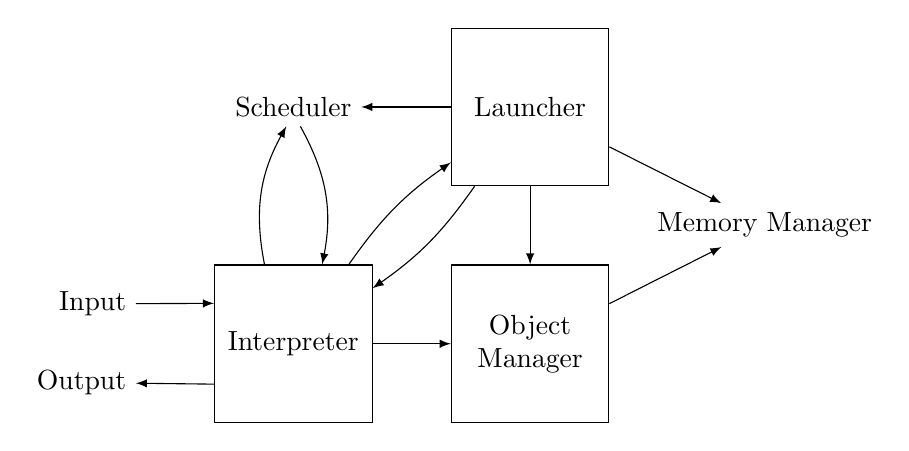
\begin{tikzpicture}
    \node[draw, minimum size=2cm, below right=2cm, align=center]
    (M) {Object\\Manager};
    \node[draw, minimum size=2cm, below=2cm]
    (I) {Interpreter};
    \node[draw, minimum size=2cm, right=2cm]
    (L) {Launcher};

    \draw[-latex, bend left=10] (I) edge (L);
    \draw[-latex, bend left=10] (L) edge (I);
    \draw[-latex] (I) edge (M);
    \draw[-latex] (L) edge (M);
    

    \node[below=1.5cm, right=4.5cm] (MM) {Memory Manager};
    \node[] (S) {Scheduler};
    \draw[-latex] (M) edge (MM);
    \draw (L) edge[-latex] (S);
    \draw (S) edge[-latex, bend left=20] (I);
    \draw (I) edge[-latex, bend left=20] (S);
    \draw (L) edge[-latex] (MM);

    \node[below=2.5cm, left=2cm] (In) {Input};
    \node[below=3.5cm, left=2cm] (Out) {Output};
    \draw[-latex] (In) to (I.153);
    \draw[-latex] (I.207) to (Out);
  \end{tikzpicture}
  \caption{The CEE model processes and their communication with each
    other and the SCJVM services}
  \label{cee-model-fig}
\end{figure}

The launcher manages the startup procedure for the SCJVM and the
execution of missions.
This involves communication with the interpreter (or C program) to
execute initialisation methods.
The interpreter then communicates back with the launcher when it
requires services that are provided by the SCJ infrastructure and API,
such as registering a schedulable object with the current mission.
Allocation of backing stores for the schedulable objects and entering
the corresponding memory areas involves communication with both the
object (or struct) manager in the CEE and the memory manager of the
SCJVM services.
The launcher must also communicate with the scheduler to indicate when
threads should be started or suspended during mission execution.

The interpreter must accept the requests to execute methods on the
main thread from the launcher, and it must also respond to requests
from the scheduler to start the other threads.
When a thread has finished execution, the interpreter signals to the
scheduler that the thread has finished so that it is no longer
scheduled.
The interpreter must also communicate with the launcher to handle
calls to methods that are provided by the SCJ infrastructure, such as
the methods to enter memory areas.
Handling of memory allocation during method execution is performed via
communication with the object manager, which then communicates with
the SCJVM memory manager.
Additionally, the interpreter communicates inputs and outputs to some
console input/output device, which is the only such device required by
the SCJ specification.
Supporting a full range of hardware connections is beyond the scope of
this work.

The interactions just described are modelled by channel
communications.
Those with the SCJVM services memory manager and scheduler use the
channels already described in
Sections~\ref{memory-manager-model-section}
and~\ref{scheduler-model-section}.
The types of values communicated by those channels are also used by
the CEE processes.
These include the type of object identifiers, $ObjectID$, the type of
thread identifiers, $ThreadID$, the type of backing store identifiers,
$BackingStoreID$, and the type of virtual machine data words, $Word$.
We also use the $ClassID$ and $MethodID$ types, which are the types of
class and method identifiers that are declared in the scheduler model
to permit the declaration of the $CEEstartThread$ channel.
Additionally, we declare a field identifier type, $FieldID$.
\begin{zed}
  [FieldID]
\end{zed}
The class, method and field identifiers may be the full names used in
Java class files or some shorter representation, such as unique
identification numbers.
In any case, type information needs to be taken into account so that
methods and fields with the same name, but different type signatures,
have different identifiers.
This is because the identifiers in Java class files include the type
information and the correct operation of method overloading relies on
it.

The channels used for communication between the CEE processes are
summarised in Figure~\ref{cee-channel-table}, with the full channel
declarations shown in Appendix~\ref{cee-model-channels}.
In addition to presenting the name and type for each channel, in the
first two columns of the table.
We also indicate which components of the CEE make use of the channel.
% L - launcher
% I - interpreter
% OM - object manager.
% I/L refers to a channel that is used by both the launcher and
% interpreter, with communications on that channel interleaved.
The channels $output$ and $input$ are used for communication with the
console device mentioned earlier.
As we do not model the console device itself, these are left as
externally visible channels when the component processes are composed
into the complete SCJVM model.
% The fact that they are external channels is indicated by the use of
% \textless{}ext.\textgreater{} in the final columns of the table.
Some channels are marked with various symbols (*, \dag{}, {}+{} and
\ddag{}) so that we can refer to them later in the text.

\begin{table}[t]
  \begin{center}
    \begin{tabular}{@{}lllll}
      \hline
      & Name & Parameter Type & \multicolumn{2}{l}{Communication} \\
      &      &                & from & to     \\
      \hline
      & $executeMethod$ & $ThreadID \cross ClassID \cross MethodID \cross \seq Word$ & L & I  \\
      & $executeMethodRet$ & $ThreadID \cross Word$ & I & L  \\
      & $continueExecution$ & $ThreadID$ & I & L \\
      & $initMainThread$ & $StackID$ & L & I \\ 
      *\dag & $register$ & $ThreadID \cross ObjectID$ & I & L \\
      %* & $registerRet$ & \textless no parameters\textgreater & L & I \\
      *\dag & $enterPrivateMemory$ & $ThreadID \cross \nat \cross ObjectID$ & I & L \\
      *\dag & $executeInAreaOf$ & $ThreadID \cross ObjectID \cross ObjectID$ & I & L \\
      *\dag & $executeInOuterArea$ & $ThreadID \cross ObjectID$ & I & L \\
      \dag & $enterPerReleaseMemory$ & $ThreadID \cross ObjectID$ & I & L \\
      {}+{} & $suspend$ & \textless no parameters\textgreater & I & L \\
      {}+{} & $suspendRet$ & \textless no parameters\textgreater & L & I \\
      {}+{} & $resumeThread$ & $ThreadID$ & I & L \\
      {}+{} & $resumeThreadRet$ & \textless no parameters\textgreater & L & I  \\
      & $output$ & $Word$ & I & \textless ext.\textgreater \\
      & $input$ & $Word$ & \textless{}ext.\textgreater{} & I \\
      & $enterBackingStore$ & $ThreadID \cross BackingStoreID$ & L & OM \\
      & $exitBackingStore$ & $ThreadID$ & L & OM  \\
      & $exitBackingStoreRet$ & $BackingStoreID \cross \boolean$ & L & OM \\
      & $getCurrentAC$ & $ThreadID$ & L & OM \\
      & $getCurrentACRet$ & $BackingStoreID$ & OM & L \\
      & $newObject$ & $ThreadID \cross ClassID$ & I/L & OM  \\
      & $newObjectRet$ & $ObjectID$ & OM & I/L  \\
      \ddag & $getClassIDOf$ & $ObjectID \cross ClassID$ & I/L & OM  \\
      \ddag & $getField$ & $ObjectID \cross FieldID$ & I & OM \\
      \ddag & $getFieldRet$ & $Word$ & OM & I \\
      \ddag & $putField$ & $ObjectID \cross FieldID \cross Word$ & I & OM \\
      \ddag & $getStatic$ & $ClassID \cross FieldID$ & I & OM \\
      \ddag & $getStaticRet$ & $Word$ & OM & I \\
      \ddag & $putStatic$ & $ClassID \cross FieldID \cross Word$ & I & OM \\
      & $addThreadMemory$ & $ThreadID \cross BackingStoreID$ & I & OM \\
      & $removeThreadMemory$ & $ThreadID$ & I & OM \\       
      \hline
    \end{tabular}
  \end{center}
  \caption{The channels used for communication between CEE processes
    before compilation. 
    In the final two columns, L refers to the launcher, I refers to
    the interpreter, OM refers to the object manager, I/L indicates a
    channel shared by the interpreter and launcher in interleaving,
    and \textless{}ext.\textgreater{} indicates and external channel.}
  \label{cee-channel-table}
\end{table}

Most of the channels are part of pairs, with one channel to
communicate a signal to begin an operation and supply any inputs, and
a return channel to communicate back when the operation has finished
and supply any outputs.
The return channel is named by appending $Ret$ to the name of the
channel used to initiate the operation.

There are some channels that deviate this pattern of having a return
channel.
The $executeMethod$ channel is used to signal to the interpreter that
it should begin execution of a method on a given thread.
The interpreter signals on $executeMethodRet$ channel when it has
finished execution of the method.
Since the launcher may need to take some action, such as exiting a
memory area, after the interpreter has finished executing a method,
the interpreter waits until it receives a signal on the
$continueExecution$ channel before continuing to execute.
Since the $continueExecution$ channel forms part of this communication
pattern, it does not have its own return channel.

Before the interpreter can execute methods on the $main$ thread, the
stack space for the $main$ thread must allocated by the launcher and
communicated to the interpreter.
This is handled by the $initMainThread$ channel, which carries the
$StackID$ for the stack space allocated for the $main$ thread.
The interpreter waits for communication on the $executeMethod$ channel
before commencing execution, so the launcher does not need to wait for
the interpreter to finish registering the $main$ thread's stack.

As mentioned above, while executing a method, the interpreter may
signal back to the launcher for handling of special methods.
The channels used for this are the ones marked with a * or a {}+{} in
Table~\ref{cee-channel-table}.
The channels marked with a * represent calls to infrastructure methods
that are part of the SCJ API.
The inputs and outputs of these methods (and hence the types of the
channels associated with them) are taken from the SCJ specification.
The channels marked with a \dag{} are methods that do not return a
value and involve execution of a method in the interpreter as part of
their handling.
Thus, the interpreter waits for a signal on the $executeMethod$
channel after signalling the launcher to handle one of these methods.
The methods marked with a \dag{} do not, therefore, require separate
return channels.
The channels marked with a + expose SCJVM scheduler operations to the
code executed in the interpreter, in order to allow for the
implementation of event handlers. 
Their types follow those of the scheduler's channels.

As mentioned previously, the $output$ and $input$ channels are used to
communicate $Word$ values to and from a console device.
The rest of the channels are used by the launcher and the interpreter
to communicate with the object manager.
The $enterBackingStore$ channel is used by the launcher to signal to
the object manager when a memory area is entered so that it can record
that the corresponding backing store has been entered.
This carries the $ThreadID$ of the thread to be entered, since the
backing stores entered are recorded separately for each thread, and
the $BackingStoreID$ of the backing store to be entered.
There is no corresponding return channel, since it is not necessary
for the launcher to wait while the object manager records the entry to
a backing store.
Similarly, the $exitBackingStore$ channel is used to signal an exit
from the backing store that is the current allocation context of the
given thread.
This does have a return channel, since the launcher must be informed
if the backing store was cleared due to no longer being in use by any
thread.
The $BackingStoreID$ of the exited backing store and a boolean value
indicating if the backing store was cleared are therefore communicated
back to the launcher on a return channel.
Additionally, the $getCurrentAC$ channel (and its return channel) is
used to obtain the $BackingStoreID$ of the backing store used as the
current allocation context for given thread from the object manager,
in order to handle some cases of entering memory areas.

The remaining channels used by the launcher to communicate with the
object manager are used by both the launcher and the interpreter.
These are the $newObject$ channel, which is used to allocate space for
new objects in the current allocation context, and the $getClassIDOf$
channel, which is used to obtain the $ClassID$ for the class of the
object associated with a given $ObjectID$.
% It is used for implementing the \texttt{new} bytecode in the
% interpreter and for creating infrastructure objects in the launcher.
% After compilation it represents a call to a method similar to
% \texttt{malloc()}.
The $newObject$ channel carries the $ThreadID$ of the current thread,
since there is a separate allocation context for each thread, and the
$ClassID$ of the class of the object to be allocated.
The object manager returns the $ObjectID$ of the newly allocated
object via the corresponding return channel.
The $getClassIDOf$ channel carries both the input and output to the
operation on the same channel, since it is a simple data accessing
operation that can be dealt with in a single communication.

The other channels used by the interpreter are the channels for
accessing fields of objects and classes.
The $getField$ channel is used for obtaining the value stored in a
given field of a given object.
It carries the $ObjectID$ of the object whose field is to be accessed
and the $FieldID$ of the field to be accessed.
The object manager then returns the $Word$ value stored in the field.
For putting a value into an object's field, the $putField$ channel is
used, which carries the $Word$ value to store in the field in addition
to the $ObjectID$ and $FieldID$ that identify the object and field to
update.
As this just updates the field and does not return any information,
there is no need for a return channel.
Channels for accessing static fields, $getStatic$ and $putStatic$, are
also provided.
These operate similarly to the channels for object fields but use
$ClassID$ values rather than $ObjectID$ values, since static fields are
attached to classes rather than objects.

The final channels used by the interpreter are the $addThreadMemory$
and $removeThreadMemory$ channels.
The $addThreadMemory$ is used to inform the object manager of a
thread's initial allocation context when the thread starts.
It carries the $ThreadID$ of the thread and the $BackingStoreID$ of
the backing store that serves as the thread's initial allocation
context.
When a thread has finished execution, it informs the object manager
via the $removeThreadMemory$ channel, which carries the $ThreadID$ of
the thread.

As mentioned earlier, some channels used by the interpreter to
communicate with the object manager are replaced with different
channels during compilation.
Those channels are marked with a \ddag{} in
Table~\ref{cee-channel-table}.
After compilation these channels are replaced with channels to obtain
the struct representing the contents of an object and to store an
object’s struct after updating it.
Note that the $getClassIDOf$ channel is shared between the launcher
and interpreter.
After compilation, the interpreter accesses a struct field storing the
$ClassID$ for an object.
However, the launcher is unaffected by the compilation and is agnostic
as to whether the program is in the form of bytecode or C code.
Therefore, the launcher continues to use the $getClassIDOf$ channel
after compilation, which represents a service offered by the object
manager or struct manager to obtain the $ClassID$ by whatever means
are appropriate to the form of the object.
As an optimisation in an implementation, the launcher could be changed
to access struct fields in the same way as the interpreter.
We discuss the form of field accesses in the C code and the channels
used for them in more detail in
Sections~\ref{cee-struct-manager-subsection}
and~\ref{cee-c-program-subsection}.

%\input{../../SCJ-VM/James/LIchans.zed}

%\input{../../SCJ-VM/James/memory_chans.zed}


Next, in Section~\ref{cee-launcher-section}, we describe our model of
the launcher.
We then detail the bytecode interpreter model in
Section~\ref{cee-interpreter-section}, and the C code model in
Section~\ref{cee-c-code-section}.

\section{Launcher}
\label{cee-launcher-section}

As mentioned in the previous section, the launcher is the component of
the CEE that manages the SCJVM startup and coordinates mission
execution.
It is described by the $Launcher$ process.

The launcher remains unaffected throughout the compilation strategy,
because it is agnostic to the class and bytecode information.
However, the launcher must know where to begin execution, so it takes
a parameter, $safeletClass$, which is the $ClassID$ of the
\texttt{Safelet} class.
This can be seen in the the $Launcher$ process definition, the
beginning of which is shown below.

Class initialisers must be executed as part of the SCJVM startup
procedure.
The order in which they are executed is determined by the dependencies
between class initialisers and classes, and is passed to the
$Launcher$ process as a second parameter, $initOrder$, which is a
sequence of $ClassID$s.
\begin{circus}
  \circprocess Launcher \circdef safeletClass : ClassID; initOrder : \seq ClassID \circspot \circbegin
\end{circus}

In what follows, we describe the definition of $Launcher$, focusing on
the aspects relevant for the compilation.
The complete definition can be found in
Appendix~\ref{launcher-appendix}.

The state of the $Launcher$ is divided into three parts.
The first part contains the identifiers of the objects that form the
SCJ mission model, so that the $Launcher$ can call methods of those
objects during SCJVM startup.
The second part contains information on the memory-area objects of
the program, including the relationship between the memory-areas and
the backing stores they represent, so that methods for entering and
exiting memory-areas can be handled.
The final part of the state describes the relationship between the
schedulable objects of SCJ and the threads used by the CEE so that the
threads can be started when mission execution begins.

We use separate Z schemas to specify each part of the state.
The first part is described by the $MissionManager$ schema, shown
below.
It contains the identifiers of three objects:
\begin{itemize}
\item $safelet$, the instance of the class implementing the
  \texttt{Safelet} interface for the program;
\item $missionSequencer$, the mission sequencer
  returned by the safelet's \texttt{getSequencer()} method; and
\item $currentMission$, the mission that is currently executing.
\end{itemize}
Methods of these objects are called at various points throughout SCJVM
startup and mission execution.
\begin{schema}{MissionManager}
  safelet, missionSequencer, currentMission : ObjectID
\end{schema}

The second part of the $Launcher$'s state is described by the
$MemoryAreaManager$ schema below.
It contains the identifiers of the memory-area objects for the
immortal memory, $immortalMemory$, and mission memory,
$missionMemory$.
There is a map, $backingStores$, that relates these identifiers and
the identifiers of the other memory-area objects, to the identifiers
of the backing stores they represent.
We also record the backing store identifiers of the per-release
memories for each thread in the $perReleaseMemories$ map.
Finally, to make sure that nested private memories can be reused,
there is a map from backing store identifiers to the identifiers of
private backing stores they contain, $privateMemoryMap$.
\begin{schema}{MemoryAreaManager}
  immortalMemory, missionMemory : ObjectID \\
  backingStores : ObjectID \finj BackingStoreID \\
  perReleaseMemories : ThreadID \finj BackingStoreID \\
  privateMemoryMap : BackingStoreID \finj BackingStoreID
\where
  \cdots
\end{schema}
Each of the maps in the $MemoryAreaManager$ is injective, since each
memory-area object has a distinct backing store and memory-areas
cannot share a nested private memory-area.
The invariants of $MemoryAreaManager$ are elided above. 
They ensure that each memory-area object has a corresponding backing
store in $backingStores$, and that areas which are not nested private
memories do not appear in the range of $privateMemoryMap$.

The final part of the state is specified in the $SchedulableManager$
schema below.
It contains a map, $schedulableThreads$, from the identifiers of
schedulable objects to the identifiers of the threads associated with
them.
This map must be injective, since every schedulable object has a
separate thread.
\begin{schema}{SchedulableManager}
  schedulableThreads : ObjectID \finj ThreadID
\end{schema}

The state of the process is then the conjunction of these three
schemas.
\begin{circusaction}
  \circstate LauncherState == MissionManager \land MemoryAreaManager \land SchedulableManager
\end{circusaction}

The $Launcher$ state is initialised as described in $LauncherInit$,
which is shown below.
The object identifiers are initialised to the $null$ identifier.
They are later filled with non-$null$ identifiers as the corresponding
objects are created during SCJVM execution.
Similarly, each of the maps is initialised to the empty set.
\begin{schema}{LauncherInit}
	LauncherState~'
\where
	\{ safelet', missionSequencer', currentMission', immortalMemory', missionMemory' \} \\
	\t1 {} \subseteq \{ null \} \\
	backingStores' = \emptyset \\
	perReleaseMemories' = \emptyset \\
	privateMemoryMap' = \emptyset \\
	schedulableThreads' = \emptyset
\end{schema}

The main action of the $Interpreter$ proceeds as shown below.
The state is first initialised as described by $LauncherInit$ and then
the actions $Startup$ and $RunNextMission$ follow in sequence.
$Startup$ defines the SCJVM startup procedure that must be performed
once at the start of SCJVM execution, whereas $RunNextMission$ defines
the procedure that must be performed for each mission run.
We do not handle mission termination in our $Launcher$ model.
This is because the SCJ mission termination procedure has almost no
effect on our compilation strategy; a single mission is sufficient for
our examples to evaluate the compilation strategy.
A formal account of it is available elsewhere~\cite{cavalcanti2013,
  luckcuck2016, zeyda2011}. 
Thus, $RunNextMission$ is only executed once.
\begin{circusaction}
  \circspot \lschexpract LauncherInit \rschexpract \circseq Startup \circseq RunNextMission
\end{circusaction}

The definition of $Startup$ is shown below.
It performs a number of actions in sequence, following the startup procedure for an SCJVM:
\begin{itemize}
\item creating the main thread's stack and passing on the
  $initMainThread$ channel, in $MakeMainStack$;
\item executing the class initialisers in the order given in
  $initOrder$, in $RunClassInitialisers$;
\item creating the immortal memory object that corresponds to the root
  backing store and storing it in $immortalMemory$, in
  $CreateImmortalMemory$;
\item creating the \texttt{Safelet} object and storing it in
  $safelet$, in $CreateSafelet$;
\item calling the \texttt{immortalMemorySize()} and
  \texttt{globalBackingStoreSize()} methods of the $safelet$, and
  checking that the size of the root backing store matches those
  values, in $CheckImmortalMemory$ and $CheckRemainingBackingStore$;
\item calling the \texttt{initializeApplication()} method of the $safelet$, in $InitializeApplication$;
\item calling the $safelet$'s \texttt{getSequencer()} method and
  storing the returned value in $missionSequencer$, in $GetSequencer$;
  and
\item creating the $missionMemory$ object with its corresponding backing store, in $CreateMissionMemory$.
\end{itemize}
\begin{circusaction}
  Startup \circdef MakeMainStack \circseq RunClassInitialisers \circseq CreateImmortalMemory \circseq CreateSafelet \circseq \\
  \t1 CheckImmortalMemory \circseq CheckRemainingBackingStore \circseq InitializeApplication \circseq \\
  \t1 GetSequencer \circseq CreateMissionMemory
\end{circusaction}

$RunNextMission$ begins with calling the \texttt{getNextMission()}
method of $missionSequencer$, in the action $GetNextMission$.
The returned mission is stored in $currentMission$.
Its \texttt{missionMemorySize()} method is then executed, and the
backing store of $missionMemory$ is resized to match, in
$ResizeMissionMemory$.
Next, in $InitializeMission$, the mission's \texttt{initialize()}
method is executed, during which the schedulable objects for the
mission are registered.
Afterwards, in $InitialiseAndStartThreads$, the registered schedulable
objects have their stacks and backing stores created, after which the
threads for all the schedulable objects are started.
Finally, in $WaitForExecution$, the $main$ thread suspends itself and
the $Launcher$ then waits, handling special methods for the threads of
the program when necessary.
Since termination is not handled, this phase of the program continues
indefinitely.
\begin{circusaction}
  RunNextMission \circdef GetNextMission \circseq ResizeMissionMemory \circseq InitializeMission \circseq \\
  \t1 InitialiseAndStartThreads \circseq WaitForExecution
\end{circusaction}

During these actions, methods are executed using the channels
$executeMethod$, $executeMethodRet$ and $continueExecution$, discussed
earlier.
The identifiers of the methods, which may be standard methods from the
SCJ API, or implementation-defined API methods required by the
launcher, are represented by constants in the model.
Although most of the methods used by the $Launcher$ are executed
simply by communicating on each of the channels mentioned above in
turn, as noted above, in $InitializeMission$, the
\texttt{initialize()} method of a mission requires handling of the
\texttt{register()} method for each schedulable object.
We must also provide handling for other special methods.
This is done in the $HandleSpecialMethodsMainLoop$ action below, which
offers handling of the special methods while waiting for return from
the \texttt{initialize()} method on the $executeMethodRet$ channel.
A similar action, without the final choice accepting
$executeMethodRet$, is used to handle special methods in
$WaitForExecution$.
\begin{circusaction}
  HandleSpecialMethodsMainLoop \circdef \circval memoryEntries : ThreadID \fun \nat; \circres retVal : Word \circspot \\
  \t1 (\Extchoice t : ThreadID \circspot \\
  \t2 EnterMemory(t) \circseq \\
  \t2 HandleSpecialMethodsMainLoop(memoryEntries \oplus \{ t \mapsto memoryEntries~t + 1 \}, retVal)) \\
  \t1 {} \extchoice {} \\
  \t1 (\Extchoice t : ThreadID \circspot \\
  \t2 \lcircguard memoryEntries~t > 0 \rcircguard \circguard ExitMemory(t) \circseq \\
  \t2 HandleSpecialMethodsMainLoop(memoryEntries \oplus \{ t \mapsto memoryEntries~t - 1 \}, retVal)) \\
  \t1 {} \extchoice {} \\
  \t1 ((Register \extchoice Suspend \extchoice Resume) \circseq \\
  \t2 HandleSpecialMethodsMainLoop(memoryEntries, retVal)) \\
  \t1 {} \extchoice {} \\
  \t1 (\lcircguard \forall t : ThreadID @ memoryEntries~t = 0 \rcircguard \circguard {} \\
  \t2 executeMethodRet?thr \prefixcolon (thr = main) ?r \then continueExecution!main \then retVal := r)
\end{circusaction}
$HandleSpecialMethodsMainLoop$ takes a value parameter,
$memoryEntries$, which is a map recording how many times a memory area
has been entered for each thread.
It also take a value parameter, $retVal$, which captures the return
value from the execution of the method on the $main$ thread.
It offers a choice of handling a memory-area entry, handling the
corresponding memory-area exit, handling a special method that does
not enter memory-areas, or accepting return from the execution of the
method on the $main$ thread (handled in the usual way using
$executeMethodRet$ and $continueExecution$, with the return value
stored in $retVal$).

$HandleSpecialMethodsMainLoop$ handles memory-area entering
methods, which execute another method after entering a memory-area,
during which further special methods may be called.
Each entry to a memory-area must be matched by a corresponding exit
from the memory-area when this extra method execution returns.
Thus, the entries to memory-areas are tracked in the $memoryEntries$
map.

The number stored in $memoryEntries$ for a thread identifier $t$ is
incremented after handling a memory-area entry on that thread as
described in $EnterMemory(t)$.
Similarly, it is decremented after handling exit from the memory-area
in $ExitMemory(t)$, which is only offered if the value is already
greater than zero.
After handling memory-area entry or exit, or another special method
(handled in the actions $Register$, $Suspend$ and $Resume$),
$HandleSpecialMethodsMainLoop$ recurses to allow further special
methods to be handled.
The return from the top-level method execution on the $main$ thread is
only permitted once all memory areas have been exited and
$memoryEntries$ is zero for all threads.

To illustrate how the nested method execution after memory-area entry
is performed, we show the $ExecuteInAreaOf$ action below, which is one
of the actions offered in external choice in $EnterMemory$, along with
actions to handle other memory-area entering operations.
$ExecuteInAreaOf$ takes a thread identifier $thread$ as a parameter
and only accepts communications from that thread, so that we can
separate out memory-area entries for each thread.
The identifier of a \texttt{Runnable} object, $runnable$, is received
via the $executeInAreaOf$ channel, which is the object that indicates
the method to be executed in the memory-area. 
Such an identifier is received for all of the memory-area entering
methods.
In the case of $ExecuteInAreaOf$, another identifier, $object$, is
also received and a $FindBackingStore$ action is used to communicate
with the memory manager to determine its backing store.
This backing store is then entered, via communication on the
$enterBackingStore$ channel.
The class of the $runnable$ object is determined and its
\texttt{run()} method (represented here by the $run$ identifier) is
executed by signalling on the $executeMethod$ channel.
No communication on the $executeMethodRet$ channel is waited for in
this action, because it is handled separately in the $ExitMemory$
action since other special methods (including further memory entries)
may occur inbetween.
\begin{circusaction}
  ExecuteInAreaOf \circdef \\
  \t1 \circval thread : ThreadID \circspot \circvar runnable, object : ObjectID; bs : BackingStoreID \circspot \\
  \t1 executeInAreaOf?t \prefixcolon (t = thread) ?obj?r \then object, runnable := obj, r \circseq \\
  \t1 FindBackingStore(object, bs) \circseq \\
  \t1 enterBackingStore!thread!bs \then getClassIDOf!runnable?runnableClass \\
  \t1 {} \then executeMethod!thread!runnableClass!run!(\langle runnable \rangle) \then \Skip
\end{circusaction}
The return from the \texttt{run()} method, and the exit from the
memory-area, is specified by the $ExitMemory$ action below.
This, as with the $ExecuteInAreaOf$ action, takes a $thread$
parameter.
A return from a method executing on that thread is accepted on the
$executeMethodRet$ channel, and its return value is discarded as the
\texttt{run()} method is \texttt{void}.
The exit from the memory-area is then performed using the
$exitBackingStore$ and $exitBackingStoreRet$ channels.
The $Launcher$ state may afterwards be updated to account for the
exited memory-area being cleared (due to no longer being in use by any
thread), which is specified in the $ClearPrivateMemory$ schema.
After the exit from the memory-area has been handled, the $Launcher$
signals that normal execution on $thread$ may continue using the
$continueExecution$ channel.
\begin{circusaction}
  ExitMemory \circdef \circval thread : ThreadID \circspot \\
  \t1 executeMethodRet?t \prefixcolon (t = thread) ?void \\
  \t1 {} \then exitBackingStore!thread \then exitBackingStoreRet?bsid?isCleared \then {} \\
  \t1 \circif isCleared = \true \circthen \lschexpract ClearPrivateMemory[bsid/toClear?] \rschexpract \\
  \t1 {} \circelse isCleared = \false \circthen \Skip \\
  \t1 \circfi \circseq continueExecution!thread \then \Skip
\end{circusaction}

The \texttt{register()} method also needs to execute a method in the
interpreter to obtain a thread's priority.
Further special methods are not handled in this case, since the method
to obtain a thread's priority is expected to be a simple method that
does not call special methods.

This handling of special methods is used by the interpreter process
(or C program, after compilation), which must communicate with the
$Launcher$ when such methods are encountered.
To allow for the behaviour of executing methods after entering memory
areas (or during the \texttt{register()} method), the interpreter must
also be prepared to execute another method after signalling to the
$Launcher$.
This is transformed to nested method executions during the compilation
strategy in order to preserve the communication pattern with the
$Launcher$.
We describe in more detail how this communication is performed in the
interpreter in Section~\ref{cee-interpreter-subsection}, and in C
program in Section~\ref{cee-c-program-subsection}.
In the next section, we describe the bytecode interpreter, which,
along with the $Launcher$, forms the CEE before the application of the
compilation strategy.

% \input{../../SCJ-VM/James/launcher.zed}

\section{Bytecode Interpreter Model}
\label{cee-interpreter-section}

This section describes the bytecode interpreter that handles execution
of an SCJ bytecode program.
Its model is composed of two processes:~the model of the object
manager, $ObjMan$, and the model of the interpreter itself,
$Interpreter$.
These are composed together in parallel with the $Launcher$ to form
the complete core execution environment, $CEE$, as shown below.
The synchronisation sets and channel hidings, omitted here, are
consistent with the communication patterns shown in
Table~\ref{cee-channel-table}.
% The parameters of each of the components, including the classes, $cs$,
% and bytecode instructions, $bc$, which are explained later in this
% section, become parameters of $CEE$.
\begin{circus}
  CEE(cs,bc,sid,initOrder) \circdef ObjMan(cs) \parallel
  Interpreter(cs,bc) \parallel Launcher(sid,initOrder)
\end{circus}
$CEE$ is parametrised by values that characterise a particular
program:~$bc$, recording the bytecode instructions, $cs$, recording
information about the classes in the program, $sid$, recording the
identifier of the \texttt{Safelet} class, and $initOrder$, a sequence
of class identifiers indicating in which order the classes should be
initialised.
These parameters are passed to the components that use them.
The $sid$ and $initOrder$ parameters have been explained in
Section~\ref{cee-launcher-section}. 
We describe the $cs$ and $bc$ later in this section where the
processes that use them are described.

$ObjMan$ manages the cooperation between the SCJ program and the SCJVM
memory manager.
This includes the representation of objects, since the SCJVM memory
manager is agnostic as to the structure of objects and objects are
shared between threads of the program.
$ObjMan$ also tracks the current memory area for each thread so that
objects can be allocated in the correct memory area.

$Interpreter$ and $Launcher$ define the control flow and semantics of
the SCJ program.
The interpreter is for a representative subset of Java bytecode that
covers stack manipulation, arithmetic, local variable manipulation,
field manipulation, object creation, method invocation and return, and
branching. 
This covers the main concepts of Java bytecode.
We do not include instructions for different types as that would add
duplication to the model while yielding no additional verification
power. 
We also do not include exception handling as SCJ programs can be
statically verified to prove that exceptions are not
thrown~\cite{kalibera2010,marriott2014}. 
Furthermore, reliance on exceptions to handle errors has been
discouraged by an empirical study due to the potential for errors in
exception handling~\cite{sawadpong2012}. 
Errors caused in the SCJVM by an incorrect input program are
represented by abortion.

Within $Interpreter$, there is one process for each thread identifier
in the set of possible thread identifiers, with the exception of the
$idle$ thread, which performs no execution.
Each of these processes represents an interpreter for a separate
thread, with thread switches coordinated by communication between
threads.
They begin with state initialisation, followed by a choice of separate
behaviours for the $main$ thread and all other threads.
The $main$ thread offers a choice of executing a method in response to
a signal from the $Launcher$ or switching to another thread.
The other threads wait for a signal from the scheduler instructing
them to start execution, after which they wait for the scheduler to
indicate they have been switched to and proceed to execute a method.

The execution of a method is performed in the same way for all
threads, repeatedly handling individual bytecode instructions until
all methods on the call stack have been returned from.
Inbetween bytecode instructions, the scheduler is polled to check for
thread switches.
After method execution has finished, the $Launcher$ and the scheduler
are signalled as appropriate, and the thread's process returns to the
start of its behaviour.

Next, in Section~\ref{cee-bytecode-subset-subsection}, we give an
informal description of the bytecode instructions handled in our model
and the ways in which their SCJ semantics differ from that of standard
Java.
In Section~\ref{cee-classes-subsection}, we describe our model of Java
class information that is used by both $ObjMan$ and $Interpreter$.
The $ObjMan$ component is then described in
Section~\ref{cee-object-manager-subsection} and $Interpreter$ is
described in Section~\ref{cee-interpreter-subsection}.

\subsection{Bytecode Subset}
\label{cee-bytecode-subset-subsection}

We model a subset of Java bytecode sufficient to express a wide
variety of SCJ programs and illustrate how further features may be
added, but small enough to permit effective reasoning.
The subset has been chosen by considering the bytecode generated from
a simple SCJ program and removing instructions similar to those
already in the subset.
This ensures the model is not unnecessarily complicated with trivial
or redundant instructions, so we can concentrate on the instructions
that are most of interest in creating the compilation strategy.
The bytecode instructions in our subset are described in
Table~\ref{bytecode-subset-table}.

\begin{table}
  \centering
  \begin{tabular}{llp{8.5cm}}
    \hline
    Instruction & Parameter & Description \\
    \hline
    \texttt{aconst\_null} & (none) & 
    Pushes a null object reference onto the operand stack.
    \\
    \texttt{aload} & local variable index &
    Loads the value from a specified local variable and pushes it
    onto the operand stack.
    \\
    \texttt{areturn} & (none) &
    Returns from the current method, pushing the value on top of the
    current method's operand stack onto the operand stack of the
    method returned to.
    \\
    \texttt{astore} & local variable index &
    Pops a value from the operand stack and stores it in the specified
    local variable.
    \\
    \texttt{dup} & (none) &
    Duplicates the value on top of the operand stack.
    \\
    \texttt{getfield} & constant pool index &
    Pops an object reference from the operand stack, gets the value of
    the field specified by the identifier at the given constant pool
    index for the referenced object, and pushes it onto the operand
    stack.
    \\
    \texttt{getstatic} & constant pool index &
    Gets the value of the static field specified by the field and
    class identifiers at the given constant pool index, and pushes it
    onto the operand stack.
    \\
    \texttt{goto} & program address &
    Unconditionally branches to the given program address.
    \\
    \texttt{iadd} & (none) &
    Pops two integer values from the operand stack, adds them, and
    pushes the result onto the operand stack.
    \\
    \texttt{iconst} & integer value &
    Pushes the given integer value onto the operand stack of the
    current method.
    \\
    \texttt{if\_icmple} & program address &
    Pops two integer values from the operand stack, and branches to
    the given program address if the second value popped is less than
    or equal to the first value.
    \\
    \texttt{ineg} & (none) &
    Pops an integer value from the operand stack, negates it, and
    pushes the negated value onto the operand stack.
    \\
    \texttt{invokespecial} & constant pool index &
    Gets the method and class identifier at the given constant pool
    index and invokes the specified method of the specified class,
    popping the method's arguments, including a \texttt{this} object
    reference, from the operand stack.
    \\
    \texttt{invokestatic} & constant pool index &
    Gets the method and class identifier at the given constant pool
    index and invokes the specified static method of the specified
    class, popping the method's arguments from the operand stack.
    \\
    \texttt{invokevirtual} & constant pool index &
    Gets the method and class identifier at the given constant pool
    index, pops the arguments of the specified method, including a
    \texttt{this} object reference, from the operand stack, and
    invokes the specified method of the class of referenced object.
    \\
    \texttt{new} & constant pool index &
    Allocates a new object of the class specified by the identifier at
    the given constant pool index and pushes a reference to the new
    object onto the operand stack.
    \\
    \texttt{putfield} & constant pool index &
    Pops an object reference and value from the operand stack and
    stores the value in the field specified by the identifier at the
    given constant pool index for the referenced object.
    \\
    \texttt{putstatic} & constant pool index &
    Pops a value from the operand stack and stores the value in the
    static field specified by the field and class identifiers at the
    given constant pool index.
    \\
    \texttt{return} & (none) &
    Returns from a method with no return value.
    \\
    \hline
  \end{tabular}
  \caption{The instructions in our bytecode subset}
  \label{bytecode-subset-table}
\end{table}

Java bytecode instructions operate over a state that records
information on all loaded classes, a stack frame, and the object data
residing in memory.
Various pieces of class information are required for execution of
bytecode instructions, but a constant pool, which stores all the
constants and names required by the class, is the main information
used.

The constant pool contains references to classes, methods and fields
used by the bytecode instructions in the class, as well as constant
values used in the code.
The form of the constant pool is a large array.
Indices into this array are used as parameters to instructions
requiring information from the constant pool.
For example, the \texttt{getfield} and \texttt{putfield} instructions
take constant pool index parameters pointing to a reference to a field
whose value should be obtained or set.
Other class information used at runtime includes information on fields
and methods belonging to the class, which is required for creation of
objects and invocation of methods.

The frame stack forms the second part of the JVM manipulated by
bytecode instructions and consists of a series of frames that contain
the runtime information for each invocation of a method.
When a method is invoked, a new stack frame is created for it and
pushed onto the frame stack, and when the method returns, the stack
frame is popped from the stack.

Each stack frame contains an operand stack, which is used to store
values manipulated by bytecode instructions, and an array of local
variables.
Most bytecode instructions manipulate the operand stack in some way,
popping arguments from it, pushing results to it or performing
specific operations upon it.

The local variables are used to store the arguments of a method and
the results of computations performed on the operand stack.
Operations are not performed directly on the local variables, so the
only bytecode instructions that affect them are those for moving
values between the operand stack and the local variables
(\texttt{aload} and \texttt{astore} are examples of such
instructions).

Some bytecode instructions also manipulate objects, which in our case
reside in backing store memory.
Such instructions include \texttt{new}, which creates objects, and
\texttt{getfield}, which gets the value from a field of an object.
In our choice of instructions for the subset, we mainly focus on
manipulation of objects and method invocation, since those are core
concepts of Java bytecode and require special handling by the
compilation strategy.

The instruction \texttt{dup} is included as an example of a simple
instruction that operates on the operand stack.
It has been chosen for its frequent occurrence in object initialisation.
Other instructions that do simple operand stack manipulation,
including the arithmetic instructions, can be specified similarly.

We also include a few arithmetic instructions as an example of how
integers are handled.
Specifically, we include the integer addition operation,
\texttt{iadd}, as an example of a binary operation, and the integer
negation operation, \texttt{ineg}, as an example of an unary
operation.
We do not include operations for floating point values since the
operations upon them are not substantially different from those on
integers at the level of modelling and compilation.
The model can be easily extended to include more integer operations.

Instructions that create object references (the \texttt{new} and
\texttt{aconst\_null} instructions), pass them around (\texttt{aload},
\texttt{astore}, \texttt{areturn}, etc.), and permit
field accesses (\texttt{getfield} and \texttt{putfield}) are also
included to allow the full range of object manipulations.
We also provide instructions for \texttt{static} field accesses
(\texttt{getstatic} and \texttt{putstatic}) since they are of use in
sharing data between different parts of the program.
However, arrays are not included as they require additional
instructions and can be emulated, albeit inefficiently, with the
instructions given here.

Both the \texttt{invokevirtual} and \texttt{invokespecial}
instructions, which invoke methods on objects, are included.
The \texttt{invokevirtual} instruction looks up the method to invoke
in the method table for the class of the object that the method is
invoked on.
The \texttt{invokespecial} instruction, on the other hand, uses the
class identifier supplied in the method reference pointed to by the
parameter of the instruction when looking up the method.
The \texttt{invokestatic} instruction, for invoking \texttt{static}
methods of classes, is similar to \texttt{invokespecial}, but does not
supply a \texttt{this} object parameter, whereas
\texttt{invokevirtual} and \texttt{invokespecial} pop \texttt{this}
from the stack as an extra argument.

The \texttt{goto} and \texttt{if\_icmple} instructions are provided as
examples of control flow instructions, with \texttt{goto} representing
an unconditional branch and \texttt{if\_icmple} representing a
conditional branch.
Other forms of conditional branch may be implemented in a similar
fashion to \texttt{if\_icmple}, but we do not include those in our
subset since \texttt{if\_icmple} is sufficient to represent most
control flow structures.
Although \texttt{goto} could be represented as a special case of
\texttt{if\_icmple}, we include it as a separate instruction due to
its frequent use in conjunction with \texttt{if\_icmple} to implement
loops.

We do not handle exceptions; errors in the SCJVM are instead handled
by simply aborting execution.
SCJ programs can be statically verified to prove that exceptions will
not be thrown~\cite{kalibera2010,marriott2014}.
Furthermore, reliance on exceptions to handle errors has been
discouraged by an empirical study due to the potential for errors in
exception handling~\cite{sawadpong2012}.
The bytecode instructions that relate to throwing and catching
exceptions are, therefore, not included in our bytecode subset.

As a simplifying assumption, we consider that all values consist of
only a single virtual machine word.
This means that \texttt{long} and \texttt{double} values are not
handled.
Any SCJ API methods that take \texttt{long} or \texttt{double}
arguments are viewed as taking \texttt{int} or \texttt{float} instead.
The reason for this assumption is that handling of two word values
makes little difference at the level of the formal model and our
approach can be easily extended to deal with more types.

Further, we do not make a distinction between the different virtual
machine types in our bytecode instructions.
This is justified as the bytecode instructions simply handle values as
32-bit words, with the type information only used for typechecking
during bytecode validation. 
The code passed into the core execution environment is assumed to have
already passed, which may be done by a separate
component~\cite{klein2003, stark2001, coglio2000, xavier2003}). 
Since many of the instructions behave the same for different types, we
only include those instructions that handle values as object
references.
We would introduce a lot of duplication in the model if, for example,
both the \texttt{areturn} and \texttt{ireturn} instructions were to be
included.

Because we are considering bytecode arising from an SCJ program, some
requirements of SCJ permit further simplifications to our bytecode
subset.
The \texttt{invokedynamic} instruction performs method invocation with
runtime typechecking, mainly for the purpose of implementing
dynamically-typed languages targeting the JVM (though it is also used
to implement the lambda expressions introduced in Java 8).
It is not included in our subset as it does not allow static
typechecking and so should not be used for SCJ.

The requirement for all classes to be loaded at startup greatly
simplifies the semantics of several instructions, since dynamic class
loading does not need to be considered.
It also means that method lookup tables can be precomputed.
This means that the semantics of the \texttt{invokevirtual} and
\texttt{invokeinterface} instructions are the same, since they both
invoke a method on an object, using the object's class as the class
for method lookup.
They, therefore, do not both need to be included and so we have not
included the \texttt{invokeinterface} instruction, since it exists
only to optimise method lookup.

In terms of concurrency considerations, we are assuming our SCJVM to
be single processor, and so we do not need to have more than one
interpreter.
As we see later, the interpreter's threads are modelled using separate
\Circus{} processes, but execution only occurs on one at a time.
We also assume that thread switches can only occur between bytecode
instructions in the interpreter.
This is justified since bytecode instructions should appear to be
atomic.
An implementation may be non-atomic as long as the externally visible
sequence of events is the same as for the model with atomic
instructions.
This means that instructions requiring communication with other
components of the SCJVM, such as \texttt{new}, which communicates with
the memory manager, must be atomic since that they affect shared
state.

Having described our bytecode subset and the assumptions we are
making, we now proceed to describe our model of Java classes in the
next section.

\subsection{Classes}
\label{cee-classes-subsection}

In our model, information about the Java classes that form the program
is recorded in a map, $cs$, that is provided as a parameter to $CEE$.
The $cs$ map associates $ClassID$s with records of a schema type
$Class$ defined as the conjunction of three schemas.
The first schema, $ClassConstantPool$ contains components that
represent the constant pool and indices into the constant pool.
The second schema, $ClassMethods$, represents information on the
methods in the class.
The final schema, $ClassFields$, is our model for information on the
fields in the class.

The components of $ClassConstantPool$ are $constantPool$, the constant
pool itself, and some indices into $constantPool$:~$this$, referencing
the current class, $super$, referencing the current class' superclass,
and $interfaces$, a set of indices referencing the interfaces
implemented by the current class.
\begin{schema}{ClassConstantPool}
  constantPool : CPIndex \pfun CPEntry \\
  this, super : CPIndex \\
  interfaces : \finset CPIndex
\where
  % the null constant pool entry is not a valid constant pool entry
  nullCPIndex \notin \dom constantPool \\
  % this, super and interfaces must all be valid constant pool indicies (except that super may be null)
  \{this\} \cup (\{ super\} \setminus \{nullCPIndex\}) \cup interfaces \subseteq \dom constantPool \\
  % this, super and interfaces must point to ClassRefs
  constantPool \limg \{this, super\} \cup interfaces \rimg \subseteq \ran ClassRef
\end{schema}
% \begin{schema}{Class}
%   constantPool : CPIndex \pfun CPEntry \\
%   this, super : CPIndex \\
%   interfaces : \finset CPIndex \\
%   methodEntry, methodEnd : MethodID \pfun ProgramAddress \\
%   methodLocals, methodStackSize : MethodID \pfun \nat \\
%   fields, staticFields : \finset FieldID
% \where
%   % the null constant pool entry is not a valid constant pool entry
%   nullCPIndex \notin \dom constantPool \\
%   % this, super and interfaces must all be valid constant pool indicies (except that super may be null)
%   \{this\} \cup (\{ super\} \setminus \{nullCPIndex\}) \cup interfaces \subseteq \dom constantPool \\
%   % this, super and interfaces must point to ClassRefs
%   constantPool \limg \{this, super\} \cup interfaces \rimg \subseteq \ran ClassRef \\
%   \dom methodEntry = \dom methodEnd = \dom methodLocals = \dom methodStackSize \\
%   \forall m : \dom methodEntry @ methodEntry~m \leq methodEnd~m \\
%   % a method's local variables must at least include space for its arguments
%   \forall m : \dom methodLocals @ methodArguments~m \leq methodLocals~m
% \end{schema}
The entries of $constantPool$ are indexed by a elements of a type
$CPIndex$.
In the JVM, the $CPIndex$ values are positive integers, but no
arithmetic or comparison is performed on constant pool indices in our
model, so we do not represent that fact.

We distinguish one particular $CPIndex$ value, a constant
$nullCPIndex$, which represents an invalid index into the
$constantPool$.
It is used as a placeholder in cases when no index is present.
For example, the class \texttt{Object} has no superclass, so the index
of the constant pool entry referencing its superclass is
$nullCPIndex$.

Each of the entries in the $constantPool$ is represented by an element
of a free type $CPEntry$, the definition of which is shown below.
It has three constructors:~$ClassRef$, representing a reference to a
$ClassID$, $MethodRef$, representing a reference to a method of a
particular class by a $ClassID$ and $MethodID$, and $FieldRef$,
representing a reference to a field of a particular class by a
$ClassID$ and $FieldID$.
\begin{zed}
  CPEntry ::= \\
  \t1 ClassRef \ldata ClassID \rdata | MethodRef \ldata
  ClassID \cross MethodID \rdata | FieldRef \ldata ClassID \cross
  FieldID \rdata
\end{zed}
Although there are other types of constant pool entry described in the
JVM specification, we do not include them in our model since some of
them are not relevant to our subset. 
Some constant pool entries are used by other constant pool entries.
For example, in the JVM specification, method references reference
another constant pool entry, which in turn contains references to
further constant pool entries with string representations of the
method's name and type.
In our model, we hide this complexity in the identifier types
$ClassID$, $MethodID$ and $FieldID$, omitting the extra constant pool
entries.

The first conjunct of the invariant of $ClassConstantPool$ requires
that $nullCPIndex$ not be in the domain of $constantPool$, since
$nullCPIndex$ is not a valid index into $constantPool$.
The second conjunct states that the indices $this$, $super$, and
$interfaces$ must be in the domain of $constantPool$, unless $super$
is $nullCPIndex$ (which is the case for the \texttt{Object} class).
Finally, the third conjunct requires that the $constantPool$ entries
at $this$, $super$ and $interfaces$ are $ClassRef$s.

The components of $ClassMethods$, shown below, are maps from
$MethodID$ values to information about each method.
The first two, $methodEntry$ and $methodEnd$, map to $ProgramAddress$
values, which are indices into a separate bytecode array representing
the start and end points of the method.
The next two components, $methodLocals$ and $methodStackSize$, map to
natural numbers giving the required number of local variables and
operand stack slots for the method.
These values are used during the compilation strategy to declare C
variables to store the local variables and operand stack values.
The final component, $staticMethods$, is a set of $MethodID$ values
for the static methods of the class.
The methods not in the $staticMethods$ are considered to be non-static
methods and must take an additional \texttt{this} argument.
\begin{schema}{ClassMethods}
  methodEntry, methodEnd : MethodID \pfun ProgramAddress \\
  methodLocals, methodStackSize : MethodID \pfun \nat \\
  staticMethods : \finset MethodID
\where
  \dom methodEntry = \dom methodEnd = \dom methodLocals = \dom methodStackSize \\
  staticMethods \subseteq \dom methodEntry \\
  \forall m : \dom methodEntry @ methodEntry~m \leq methodEnd~m \\
  % a method's local variables must at least include space for its arguments
  \t1 \land methodArguments~m + (\IF m \in staticMethods \THEN 0 \ELSE 1) \leq methodLocals~m 
\end{schema}
In addition to the components of $ClassMethods$, we declare a global
function $methodArguments$ from $MethodID$s to natural numbers, which
gives the number of arguments that each method takes.
This is a global function since each $MethodID$ encodes the type of
the method, so the number of arguments for a method can always be
determined from its identifier.
The $methodArguments$ function is also total for this reason.
We use $methodArguments$ in the invariant of $ClassMethods$, and also
in the $Interpreter$ and compilation strategy when handling method
calls.

The first conjunct of the invariant of $ClassMethods$ requires that
all the component maps have the same domain, so that all the
information must be supplied for any method present in the class.
The second conjunct requires that every $MethodID$ in $staticMethods$
be within the domains of these maps.
Finally, the third conjunct requires that, for each method, its
$methodEntry$ is before its $methodEnd$, and that its $methodLocals$
is large enough to contain its $methodArguments$, plus an extra
\texttt{this} argument for non-static methods, since each argument of
a method is stored in a local variable.

The final components of our model for class information are given in
the $ClassFields$ schema below.
It contains two sets of $FieldID$s, $fields$ and $staticFields$, which
are the identifiers of the class' object fields and static fields
respectively.
The static and non-static fields need to be distinguished so that we
know where each needs to be stored:~static variables have only one
copy for each class, whereas non-static fields are stored separately
for each instance of a class.
The $fields$ and $staticFields$ sets are required to be disjoint since
no field can be both static and non-static.
\begin{schema}{ClassFields}
  fields, staticFields : \finset FieldID
\where
  fields \cap staticFields = \emptyset
\end{schema}

The three schemas containing the different parts of the class
information are conjoined together to form $Class$, as shown below.
\begin{zed}
  Class == ClassConstantPool \land ClassMethods \land ClassFields
\end{zed}

In addition to defining $Class$, we also define functions for
extracting information from the $constantPool$ for a given $Class$, in
order to make specifying things about them easier.
Since the functions are just abbreviations of data access operations,
we omit them here.
We recall that the definitions omitted here are given in
Appendix~\ref{full-cee-model}.

We also require a way of expressing the fact that one class is a
subclass of another.
We say that a $Class$ binding, $c1$, is a direct subclass of another
class, $c2$, written $c1 \directsubclass c2$, if the $this$ identifier
of $c2$ is the $super$ identifier of $c1$ or one of its $interfaces$
identifiers.

We also define a relation, $subClassRel$, between class identifiers
$cid1$ and $cid2$ in terms of the $\directsubclass$ relation.
This requires a map from $ClassID$ to bindings of $Class$, which is
provided as a parameter to $subclassRel$.
Given such a map, $cs$, we define $(cid1,cid2) \in subclassRel~cs$ to
hold if, in $cs$, $cid1$ and $cid2$ refer to $Class$ bindings such
that $cs~cid1 \directsubclass cs~cid2$ holds.
We expand $subclassRel$ to refer to its reflexive transitive closure
so that it includes indirect subclass relationships and classes being
subclasses of themselves.
We omit the formal definitions of $\directsubclass$ and $subclassRel$
here.

The $cs$ map provided as a parameter to $CEE$ is used as the parameter
to $subclassRel$ in each of the processes that uses it.
In order for the CEE to execute the program, this $cs$ parameter must
represent a valid SCJ program, with all the necessary classes present.
If this holds, then $subclassRel$ represents the usual notion of when
a object of a Java class is assignable to a variable of a given class.

We next describe the object manager process, $ObjMan$, which uses the
$Class$ type and the $cs$ map.

\subsection{Object Manager}
\label{cee-object-manager-subsection}

The object manager, which is represented by the process $ObjMan$,
manages the objects of the SCJ program executed by the core execution
environment.
This component is necessary because the SCJVM memory manager is
agnostic to the structure of objects, which depends on the contents of
the classes supplied as part of an SCJ program.
Besides managing the creation and manipulation of objects, the object
manager tracks the current allocation context for each thread.
It ensures objects are allocated in the correct area, since the SCJVM
memory manager is also agnostic to the existence of threads.

The start of the definition of $ObjMan$ is shown below.
$ObjMan$ takes a single parameter, $cs$, which is a map from
$ClassID$s to $Class$ records containing the class information for
each of the classes in the program.
This information is used in determining the structure of the objects
for each class.
\begin{circus}
  \circprocess ObjMan \circdef cs : ClassID \pfun Class \circspot \circbegin
\end{circus}

Since the actual arrangement of an object in memory is an
implementation consideration, the amount of memory required to store
each object is implementation-defined.
It is represented here by a global function $sizeOfObject$, declared
below, which maps the information in each $Class$ to the amount of
memory required for objects of the class it represents.
\begin{axdef}
  sizeOfObject : Class \fun \nat
\end{axdef}

The objects that $ObjMan$ operates on are described by records of the
schema type $Object$ shown below.
It contains a map, $fields$, which associates the $FieldID$ for each
field of an object with a $Word$ value stored in that field.
A copy of the $Class$ information for the object's class is also
recorded in $class$.
The invariant of $Object$ requires that the domain of $fields$ be the
same as the fields given in $class$.
\begin{schema}{Object}
  fields : FieldID \pfun Word \\
  class : Class
\where
  \dom fields = class.fields
\end{schema}      

The state of $ObjMan$ is described by the schema $ObjManState$, shown
below.
Its first component is a map, $objects$, from $ObjectID$s to $Object$
records, storing the actual object data for the program.
Its second component, $backingStoreMap$, associates backing stores
with the identifiers of objects stored within them.
The third component, $backingStoreStacks$, associates to each
$ThreadID$ a sequence of $BackingStoreID$ values representing the
backing stores entered by the thread.
This is required to contain at least one value, since each thread that
is ready to execute must have a backing store, and those that are not
should not be in the domain of $backingStoreStacks$.
$ObjManState$ also stores $rootBS$, a copy of the root backing store
identifier.
The final components of $ObjManState$ are used to store the static
fields of classes.
The $staticClassFieldsID$ component is of a free type
$StaticFieldsStructID$, and may be either $Uninitialised$ or
$Initialised$ with an $ObjectID$ representing the space allocated for
the static class fields.
The values of the fields themselves are stored in the
$staticClassFields$ map.
\begin{schema}{ObjManState}
  objects : ObjectID \pfun Object \\
  backingStoreMap : BackingStoreID \pfun \finset ObjectID \\
  backingStoreStacks : ThreadID \pfun \seq_1 BackingStoreID \\
  rootBS : BackingStoreID \\
  staticClassFieldsID : StaticFieldsStructID \\
  staticClassFields : (ClassID \cross FieldID) \pfun Word
\where
  backingStoreMap \partition \dom objects \cup toSet~staticClassFieldsID \\
  \bigcup \{ t : \dom backingStoreStacks @ \ran~(backingStoreStacks~t) \} = \dom backingStoreMap \\
  rootBS \in \dom backingStoreMap \\
  staticClassFieldsID = Uninitialised \implies staticClassFields = \{\} \\
  toSet~staticClassFieldsID \subseteq backingStoreMap~rootBS
\end{schema}
The first conjunct of the invariant requires that the domain of
$objects$, plus $staticClassFieldsID$ if it is $Initialised$, is
partitioned by the $ObjectID$ sets given by $backingStoreMap$, so that
every object is allocated in exactly one backing store.
This uses a function $toSet$ to convert $staticClassFieldsID$ to a set
of $ObjectID$s.
The second conjunct requires that the domain of $backingStoreMap$ be
the identifiers of backing stores in $backingStoreStacks$, since a
backing store that is not in use is cleared and so should not have any
objects in it.
The third conjunct requires that $rootBS$ always be in the domain of
$backingStoreMap$, since that represents immortal memory, which is
never cleared.
Combined with the second conjunct, this implies that at least one
thread must have entered the $rootBS$ at all times.
The fourth conjunct ensures that $staticClassFields$ does not contain
any fields until $staticClassFieldsID$ is $Initialised$.
Finally, the fifth conjunct requires that $staticClassFieldsID$ must
be in the root backing store.

The $ObjManState$ is initialised as described in $ObjManInit$ below.
This operation takes the identifier of the root backing store as an
input, $rootBS?$.
The $objects$ map is initialised to the empty set, since there are
initially no objects in existence.
The $backingStoreMap$ initially contains only $rootBS?$, which is the
only backing store initially in existence, associated with an empty
set of object identifiers.
The $backingStoreStacks$ map is initialised to contain the $main$ and
$idle$ thread, both with $rootBS?$ as their only backing store
entered.
The $rootBS$ identifier is set to be the same as the $rootBS?$ input.
The $staticClassFieldsID$ is set to $Uninitialised$, with
$staticClassFields$ empty.
\begin{schema}{ObjManInit}
	ObjManState~' \\
	rootBS? : BackingStoreID
\where
	objects' = \emptyset \\
	backingStoreMap' = \{ rootBS? \mapsto \emptyset \} \\
	backingStoreStacks' = \{ main \mapsto \langle rootBS? \rangle, idle \mapsto \langle rootBS? \rangle \} \\
	rootBS' = rootBS? \\
	staticClassFieldsID = Uninitialised \\
	staticClassFields = \{\}
\end{schema}

The $ObjMan$ process then proceeds as described in its main action,
shown below.
It begins in $Init$ by communicating with the SCJVM memory manager to
obtain the identifier of the root backing store and then initialising
the state as described in $ObjManInit$.
The space for static fields is then allocated in
$AllocateStaticFields$, initialising $staticClassFieldsID$ and
populating $staticClassFields$ with each field mapped to $null$.
Finally, in $Loop$, the process repeatedly offers each of its services
in external choice.
\begin{circusaction}
  \circspot Init \circseq AllocateStaticFields \circseq Loop
\end{circusaction}

% The space for static fields is allocated as described in
% $AllocateStaticFields$ below.
% The static field identifiers for all the classes are collected in a
% set $staticFields$, with the class identifier for each field attached.
% Space for the static fields is then allocated by communicating with
% the memory manager.
% The static fields are allocated in the backing store for the $main$
% thread, and the size required is computed from the $staticFields$ set
% via a function $staticFieldsSize$.
% If the report received from the memory manager indicates the
% allocation was successful, then the staticFields are initialised in
% $InitStaticFields$.
% This just initialises $staticClassFieldsID$ with the $objectID$
% returned from the memory manager and sets $staticClassFields$ to map
% from each element of $staticFields$ to the $null$ word.
% If the memory manager's report indicates that an error has occured
% then the action aborts.
% \begin{circusaction}
%   AllocateStaticFields \circdef \circvar staticFields : \finset (ClassID \cross FieldID) \circspot \\
%   \t1 staticFields := \bigcup \{ cid : \dom cs @ \{cid\} \cross (cs~cid).staticFields \} \circseq \\
%   \t1 MMallocateMemory!(last~(backingStoreStacks~main))!(staticFieldsSize~staticFields) \then {} \\
%   \t1 MMallocateMemoryRet?objectID \then {} \\
%   \t2 (MMreport?r \prefixcolon (r = MMokay) \then \lschexpract InitStaticFields \rschexpract \\
%   \t2 {} \extchoice MMreport?r \prefixcolon (r = MMokay) \then \Chaos)
% \end{circusaction}

% For the creation of class objects in $MakeClassObjects$ the class
% information for each object must be supplied.
% Since the objects are representations of class information, their
% class should be the \texttt{Class} class from the standard Java API (a
% stripped-down version of which is present in SCJ).
% We represent the identifier of this class by a $ClassID$ constant
% $classClass$.
% However, since the object stores the static fields for each class, the
% $fields$ of the $Class$ information associated with $classClass$ need
% to be changed to be the correct static fields in each case.
% This is accomplished using a function $replaceClassFields$, which
% takes a $Class$ and a set of $FieldID$s, and produces a new $Class$
% with the components the same as the input $Class$, except that the
% $fields$ component is set to the input $FieldID$s.

% The $replaceClassFields$ function is used in the definition of the
% $MakeClassObjects$ action, which is shown below.
% It iterates through each $ClassID$, $cid$, in the domain of $cs$, and
% allocates an object for each one using a $MakeObject$ action that
% performs the communication with the memory manager.
% The first parameter to $MakeObject$ is the $Class$ information for the
% object, which is defined by taking the value in $cs$ associated with
% $classClass$ and using $replaceClassFields$ to replace its $fields$
% with the $staticFields$ of the $Class$ associated with $cid$.
% The second parameter is the thread in whose context the object is to
% be allocated, which in this case is the $main$ thread, since that is
% only thread that is initially eligible to run.
% Since the $main$ thread's allocation context is initially immortal
% memory, the class objects are allocated in immortal memory, ensuring
% that the static fields are available throughout the program's
% execution.
% The object identifier returned from the allocation is stored in
% $objectID$, which is stored in $classObjectMap$ associated with $cid$.
% \begin{circusaction}
%   MakeClassObjects \circdef \circvar objectID : ObjectID \circspot \\
%   \t1 \Semi cid : \dom cs \circspot \\
%   \t2 MakeObject(replaceClassFields~(cs~classClass)~(cs~cid).staticFields,main,objectID) \circseq \\
%   \t2 classObjectMap := classObjectMap \cup \{cid \mapsto objectID\}
% \end{circusaction}

% The $MakeObject$ action, used in $MakeClassObjects$, is defined
% separately below since it is also used when creating objects other
% than the class objects.
% Its first two parameters are value parameters $class$, representing
% the class information for the object, and $thread$, recording the
% current thread identifier.
% The final parameter, $objectID$, is a result parameter returning the
% identifier of the object created.
% The object is created using the \texttt{allocateMemory} service of the
% memory manager, with the allocation context being the last backing
% store entered for $thread$ in $backingStoreStacks$ and the space
% allocated determined from $class$ using $sizeOfObject$.
% If the memory manager operation is successful (as indicated by a
% report of $MMokay$), then the object is initialised as described by
% $ObjManObjectInit$, which adds it to $objects$, sets its class
% information to $class$ and initialises its fields to $null$.
% Since it is a relatively simple data operation, we omit its definition
% here.
% If the memory manager operation is not successful (for example,
% because the SCJVM is out of memory) then $ObjMan$ diverges.
% \begin{circusaction}
%   MakeObject \circdef \circval class : Class; \circval thread : ThreadID; \circres objectID : ObjectID \circspot \\
%   \t1 MMallocateMemory!(last~(backingStoreStacks~thread))!(sizeOfObject~class) \then {} \\
%   \t1  MMallocateMemoryRet?objectID \then {} \\
%   \t2 (MMreport?r \prefixcolon (r = MMokay) \then \lschexpract ObjManObjectInit \rschexpract \\
%   \t2 {} \extchoice MMreport?r \prefixcolon (r \neq MMokay) \then \Chaos)
% \end{circusaction}

After $ObjMan$ is initialised and the space for the static fields has
been created, $ObjMan$ offers services to the other components of the
$CEE$, in the $Loop$ action shown below.
The services offered by $Loop$ include $NewObject$, which creates an
object of a given class.
The $GetField$ and $PutField$ actions allow for obtaining and setting
the value of an object's field.
Similarly, $GetStatic$ and $PutStatic$ allow for obtaining and setting
the value of a class' static fields, applying the same data operations
as $GetField$ and $PutField$ to the object in $classObjectMap$.
$GetClassIDOf$ obtains the $ClassID$ for the class of an object, by
extracting the $this$ identifier from the $Class$ information for the
object.

Management of allocation contexts is provided by the remaining
services.
The first is $EnterBackingStore$, which enters a backing store for a
given thread by pushing it onto the stack in $backingStoreStacks$ for
that thread, and adding it to $backingStoreMap$ if it is not already
in its domain.
The second is the corresponding operation $ExitBackingStores$ for
exiting the current allocation context of a given thread, which means
popping it from the thread's stack in $backingStoreStacks$, and
clearing and removing the backing store from $backingStoreMap$ if no
threads are still using it.
The $AddThreadMemory$ and $RemoveThreadMemory$ services allow for
adding a thread to $backingStoreStacks$ when it starts executing, and
removing it when it finishes executing.
Finally, the $GetCurrentAC$ action obtains the current allocation
context for a given thread, which is the backing store on top of its
stack in $backingStoreStacks$.
\begin{circusaction}
  Loop \circdef (NewObject \extchoice GetField \extchoice PutField \extchoice GetStatic \extchoice PutStatic \extchoice GetClassIDOf \\
  \t1 {} \extchoice EnterBackingStore \extchoice ExitBackingStore \extchoice AddThreadMemory \\
  \t1 {} \extchoice RemoveThreadMemory \extchoice GetCurrentAC)
  \circseq Loop
\end{circusaction}

The compilation refines the structure of objects.
This means that field access operations ($GetField$, $PutField$) and
object allocation ($NewObject$) are affected.
$GetClassIDOf$ is also affected since an object's class identifier is
stored as part of its structure.
We also refine the static fields data structure, requiring the
operations upon it ($AllocateStaticFields$, $GetStatic$, $PutStatic$)
to be changed.
The management of allocation contexts is unaffected by the
compilation, but is required for managing allocation of objects, so
that they can be allocated in the correct backing store.

The definition of the $NewObject$ action is shown below.
It allocates space for an object by communicating with the memory
manager in much the same way as $AllocateStaticFields$, except that
the thread and class identifiers for the object are communicated via
the $newObject$ channel, and the size required for the object is
obtained from the class information via a $sizeOfObject$ function.
After a successful allocation, the object is added to the $objects$
map with its fields initialised to $null$, in $ObjManObjectInit$, and
the object's identifier is returned via $newObjectRet$.
\begin{circusaction}
  NewObject \circdef \circvar objectID : ObjectID \circspot \\
  \t1 newObject?thread?classID \then {} \\
  \t1 MMallocateMemory!(last~(backingStoreStacks~thread))!(sizeOfObject~(cs~classID)) \then {} \\
  \t1  MMallocateMemoryRet?objectID \then {} \\
  \t2 ((MMreport?r \prefixcolon (r = MMokay) \then \lschexpract \exists class? == cs~classID @ ObjManObjectInit \rschexpract \circseq \\
  \t3 newObjectRet!objectID \then \Skip) \\
  \t2 {} \extchoice MMreport?r \prefixcolon (r \neq MMokay) \then \Chaos) 
\end{circusaction}

We omit the definitions of the other actions of $Loop$ here. 
The full model of the object manager can be found in
Appendix~\ref{object-manager-appendix}.

Next, we discuss the $Interpreter$ process, which is the final
component of $CEE$ and handles the execution of the bytecode
instructions themselves.

\subsection{Interpreter}
\label{cee-interpreter-subsection}

The $Interpreter$ process is the final component of $CEE$ that we
present. 
It handles the execution of bytecode instructions.
The bytecode instructions it handles are those in the subset described
in Section~\ref{cee-bytecode-subset-subsection}, which in our model
are represented by the free type $Bytecode$, sketched below.
$Bytecode$ has a constructor for each bytecode instruction, with any
parameter to the instruction represented as a parameter of the
constructor.
The full definitions omitted here are in
Appendix~\ref{interpreter-appendix}.
\begin{zed}
  Bytecode ::= aconst\_null | dup | areturn | return | iadd | ineg \\
  \t1 | new \ldata CPIndex \rdata | iconst \ldata \nat \rdata | aload \ldata \nat \rdata | astore \ldata \nat \rdata | \dots
\end{zed}
The bytecode instructions are arranged in a map, $bc$, from
$ProgramAddress$ values (which are modeled by natural numbers) to
$Bytecode$ values.
The $bc$ map is passed as a parameter to the $Interpreter$ process,
along with the $cs$ map described in
Section~\ref{cee-classes-subsection}, as can be seen from its
definition shown below.
The overall structure of $Interpreter$ is a parallel composition of
$Thr$ processes representing the individual interpreter threads, with
one process for each $ThreadID$ except for $idle$.
The $bc$ and $cs$ parameters are passed to each $Thr$ process, along
with its $ThreadID$.
\begin{circus}
  \circprocess Interpreter \circdef \\
  \t1 bc : ProgramAddress \pfun Bytecode; cs : ClassID \pfun Class \circspot \\
  \t1 \Parallel t : ThreadID \setminus \{ idle \} \lpar ThrChans(t) \rpar \circspot Thr(bc, cs, t)
\end{circus}
Each $Thr(bc,cs,t)$ process synchronises on a set $ThrChans(t)$,
containing the $CEEswitchThread.t.t2$ and $CEEswitchThread.t2.t$
events for all thread identifiers $t2$.
This ensures thread switches can be handled since the two threads
involved in the thread switch (the thread switched from and the thread
switched to) synchronise on the thread switch request.
This model of the interpreter threads captures the fact that they are
conceptually running in parallel, each with their own state, and we do
not mandate a specific thread switch mechanism.

\subsubsection*{State}
% \paragraph*{State}

The state of each $Thr$ process contains the stack for the thread,
which consists of a series of stack frames, one for each method on the
call stack.
The contents of each stack frame are specified by the schema
$StackFrame$.
Its first component, $localVariables$, is a sequence of $Word$ values
representing the local variable array for the method.
Its second component, $operandStack$ represents the data stack upon
which each bytecode instruction operates.
The third component, $storedPC$, is used for storing the program
counter value as a return address when another method is invoked.
The fourth component, $frameClass$, is a copy of the $Class$
information for the class of the stack frame's method, so that the
constant pool for the class is available to the operations of $Thr$.
The fifth component, $stackSize$, stores the maximum size of the
$operandStack$ for the thread.
The final component of $StackFrame$, $baseFrame$ is a boolean value
indicating whether or not the frame was created in response to an
external request, so that it forms the base of a substack of frames.
This is used when determining whether to send a return value to the
$executeMethodRet$ channel or push it onto the previous method's
$operandStack$.
\begin{schema}{StackFrame}
  localVariables : \seq Word \\
  operandStack : \seq Word \\
  storedPC : ProgramAddress \\
  frameClass : Class \\
  stackSize : \nat \\
  baseFrame : \boolean
\where
  \# operandStack \leq stackSize
\end{schema}
The invariant of $StackFrame$ just requires the $operandStack$ to not
be larger than $stackSize$.

The state of $Thr$ is given by the schema $InterpreterState$, below.
Its first component, $frameStackID$, is the identifier of the frame
stack for the thread. 
It is of a type $Stack$, which may be $Uninitialised$ with no value,
or $Initialised$ with a $StackID$ value for the stack.
The second component, $frameStack$, represents the stack itself, which
is a sequence of $StackFrame$ bindings, with one for each method
entered.
The third component, $pc$, is the program counter for the thread.
Finally, the fourth component, $currentClass$, is a copy of the class
information for the current method.
\begin{schema}{InterpreterState}
  frameStackID : Stack \\
  frameStack : \seq StackFrame \\
  pc : ProgramAddress \\
  currentClass : Class
\where
  frameStackID = Uninitialised \implies frameStack = \emptyset \\
  % definition of currentClass (only important if the frame stack is nonempty)
  frameStack \neq \emptyset \implies currentClass = (last~frameStack).frameClass \\
  frameStack \neq \emptyset \implies (head~frameStack).baseFrame = \true \\
  % need to ensure pc is consistent with currentClass
  \exists m : MethodID | m \in \dom currentClass.methodEntry @ \\
  \t1 pc \in currentClass.methodEntry~m \upto currentClass.methodEnd~m
\end{schema}
The first conjunct of the invariant requires that there be no
$StackFrames$ on the $frameStack$ when $frameStackID$ is
$Uninitialised$.
The second conjunct defines $currentClass$ as the $frameClass$ of the
last $StackFrame$ on the $frameStack$.
This is only required when $frameStack$ is nonempty, since
$currentClass$ is unused when $frameStack$ is empty.
The third conjunct states that, if the $frameStack$ is nonempty, the
first $StackFrame$ must have $baseFrame$ set to $\true$, since it is
always the start of a substack of frames.
Finally, the fourth conjunct states that $pc$ must be in the
$ProgramAddress$ range for a method of $currentClass$, to ensure the
bytecodes are associated with the correct class information.

The state is initialised as described in a schema $InterpreterInit$.
The initialisation just sets $frameStackID$ to $Unintialised$ and the
$frameStack$ to empty.
The other state components take arbitrary values and are initialised
when the first $StackFrame$ is created, since they are unused until
then.

\subsubsection*{Behaviour}

The main action of $Thr$ is shown below. 
After the initialisation, it behaves as $MainThread$ or $NotStarted$,
depending on whether the thread represented by the $Thr$ process is
the $main$ thread or not.
$MainThread$ and $NotStarted$ make use of the same actions for
executing bytecode instructions, but they occur in different orders.
The control flow of the $Thr$ process is shown in
Figure~\ref{interpreter-flow-figure}.
\begin{circusaction}
  \circspot \lschexpract InterpreterInit \rschexpract \circseq {}
  \circblockbegin
    \lcircguard thread = main \rcircguard \circguard MainThread \\
    {} \extchoice {} \\
    \lcircguard thread \neq main \rcircguard \circguard NotStarted
  \circblockend
\end{circusaction}

\begin{figure}
  \centering
  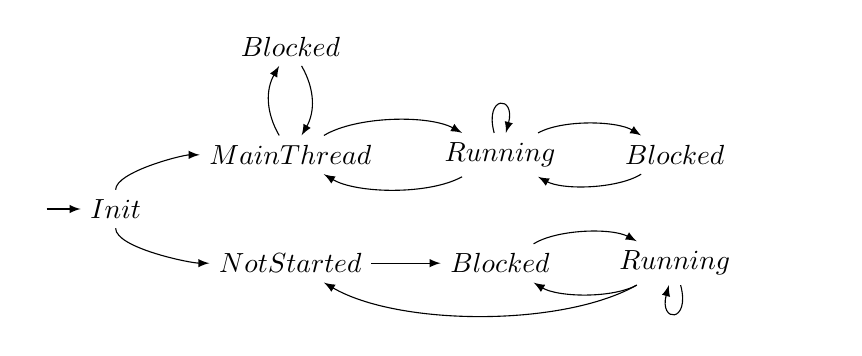
\begin{tikzpicture}
    \node at (9cm,0) (width) {};
    \node at (0,1.5cm) (height) {};

    \path (0,0) --
    node[pos=0.00] (Initxpos) {}
    node[pos=0.25] (Interpreterxpos) {}
    node[pos=0.55] (Executexpos) {}
    node[pos=0.8] (ExecuteAndPollxpos) {}
    (width);

    \path (0,0) --
    node[pos=0] (threadypos) {}
    node[pos=0.5] (Initypos) {}
    node[pos=1] (mainypos) {}
    node[pos=2] (mainBlockedypos) {}
    (height);

    \path (Initxpos |- Initypos) node (Init) {$Init$} ++(-1cm,0cm) node (start) {};
    \node at (Interpreterxpos |- mainypos) (IMn) {$MainThread$};
    \node at (Executexpos |- mainypos) (MRn) {$Running$};
    \node at (Interpreterxpos |- mainBlockedypos) (MBl) {$Blocked$};
    \node at (ExecuteAndPollxpos |- mainypos) (MB2) {$Blocked$};
    \node at (Interpreterxpos |- threadypos) (NSt) {$NotStarted$};
    \node at (Executexpos |- threadypos) (TBl) {$Blocked$};
    \node at (ExecuteAndPollxpos |- threadypos) (TRn) {$Running$};

    \draw[-latex] (start) to (Init);
    \draw[-latex] (Init) to[out=90,in=180,looseness=0.5] (IMn);
    \draw[-latex] (Init) to[out=270,in=180,looseness=0.5] (NSt);
    \draw[-latex] (IMn) to[bend left,looseness=0.7] (MRn);
    \draw[-latex] (MRn) to[bend left,looseness=0.7] (IMn);
    \draw[-latex] (MRn) to[bend left,looseness=0.7] (MB2);
    \draw[-latex] (MB2) to[bend left,looseness=0.7] (MRn);
    \draw[-latex] (IMn) to[bend left,looseness=1.0] (MBl);
    \draw[-latex] (MBl) to[bend left,looseness=1.0] (IMn);
    \draw[-latex] (NSt) to (TBl);
    \draw[-latex] (TBl) to[bend left,looseness=0.7] (TRn);
    \draw[-latex] (TRn) to[bend left,looseness=0.7] (TBl);
    \draw[-latex] (TRn) to[bend left,looseness=0.7] (NSt);
    \draw[-latex] (TRn) to[loop below] (TRn);
    \draw[-latex] (MRn) to[loop above] (MRn);
  \end{tikzpicture}
  \caption{The overall control flow of $Thr$}
  \label{interpreter-flow-figure}
\end{figure}


The $MainThread$ action is shown below.
It begins by accepting a $StackID$ from the $Launcher$ on the
$initMainThread$ channel, which is used to initialise the
$frameStackID$ state component.
It then offers a choice of executing a method on the $main$ thread in
response to a request from the $Launcher$, or switching to another
thread.
A request to start execution of a method is handled in the
$StartIntepreter$ action, which creates the $StackFrame$ for the
method.
The process then behaves as the $Running$ action, executing bytecode
instructions until the method has finished, after which the
$MainThread$ action recurses to offer the choice of method execution
and thread switch again.
If an instruction to switch to another thread from the scheduler is
received on the $CEEswitchThread$ channel, then it is only accepted if
the thread switched from is the $thread$ represented by the process.
If it is accepted, then the process behaves as $Blocked$, waiting for
a request to switch back to the thread, after which it recurses back
to offer the choice of behaviours again.
\begin{circusaction}
  MainThread \circdef initMainThread?stack \then frameStackID := Initialised~stack \circseq \circmu X \circspot \\
  \t1 \circblockbegin
  StartInterpreter \circseq Running \circseq X \\
  {} \extchoice {} \\
  CEEswitchThread?from?to \prefixcolon (from = thread) \then Blocked \circseq X
  \circblockend
\end{circusaction}

The $StartIntepreter$ action, used by $MainThread$ also handles
special methods that execute nested methods.
Its definition is shown below.
It accepts communication on the $executeMethod$ channel, requiring the
$ThreadID$ communicated to be the same as that of the current thread,
$thread$, and storing the other values communicated as $classID$,
$methodID$ and $methodArgs$.
A data operation $ResolveMethod$ is then used to determine the
appropriate class information for the method, since the method may
actually be defined in a superclass of the provided $classID$.
$ResolveMethod$ follows the method resolution rules of the JVM
specification, first checking if the class corresponding to $classID$
defines the method, then checking if one of its superclasses defines
the method, and finally looking for the method definition among its
superinterfaces.
The $Class$ information resulting from this is stored in $class$ and
used to create a new $StackFrame$ on the $frameStack$ in
$InterpreterNewStackFrame$.
The $baseFrame$ value for this stack frame is set to $\true$, since it
is being created in reponse to an external request.
\begin{circusaction}
  StartInterpreter \circdef \\
  \t1  \circvar classID : ClassID; methodID : MethodID; methodArgs : \seq Word; class : Class \circspot \\
  \t1 executeMethod?t \prefixcolon (t = thread) ?c?m?a \then classID, methodID, methodArgs := c, m, a \circseq \\
  \t1 \lschexpract ResolveMethod[cs/cs?] \rschexpract \circseq \lschexpract \exists baseFrame? == \true @ InterpreterNewStackFrame \rschexpract
\end{circusaction}

For threads other than $main$, the behaviour is described by the
$NotStarted$ action below.
It accepts a request to start the $thread$ represented by the process
from the scheduler on the $CEEstartThread$ channel.
The identifier, $bsid$, of the thread's backing store is then passed
to $ObjMan$ via the $addThreadMemory$ channel and the $stack$
identifier is used to initialise $frameStackID$.
The remaining information is stored in $classID$, $methodID$ and
$methodArgs$, and the $Class$ information is determined and a new
$StackFrame$ is created, similarly to what happends in
$StartInterpreter$. 
The process then behaves as the $Blocked$ action, waiting for an
instruction to switch to that thread, after which it behaves as the
$Running$ action, executing bytecode instructions.
When the execution of the thread's method has finished, the scheduler
is signalled on the $CEEremoveThread$ channel.
This causes the scheduler to switch to a different thread, so a thread
switch is accepted on the $CEEswitchThread$ channel.
After that, the action recurses to allow the thread to be restarted.
\begin{circusaction}
  NotStarted \circdef \\
  \t1 \circvar classID : ClassID; methodID : MethodID; methodArgs : \seq Word; class : Class \circspot \\
  \t1 CEEstartThread?toStart?bsid?stack?cid?mid?args \prefixcolon (toStart = thread) \then {} \\
  \t1 addThreadMemory!thread!bsid \then {} \\
  \t1 frameStackID, classID, methodID, methodArgs := Initialised~stack, cid, mid, args \circseq \\
  \t1 \lschexpract ResolveMethod[cs/cs?] \rschexpract \circseq \lschexpract \exists baseFrame? == \true @ InterpreterNewStackFrame \rschexpract \circseq \\
  \t1 Blocked \circseq Running \circseq CEEremoveThread!thread \then {} \\
  \t1 CEEswitchThread?from?to \prefixcolon (from = thread) \then NotStarted
\end{circusaction}

The $Blocked$ and $Running$ actions define the behaviour of threads
after they have been started.
The $Blocked$ action simply waits for a signal on the
$CEEswitchThread$ channel to switch to $thread$, after which it
terminates to allow execution in a different action to continue.
\begin{circusaction}
  Blocked \circdef CEEswitchThread?from?to \prefixcolon (to = thread) \then \Skip
\end{circusaction}

The $Running$ action, shown below, executes the bytecode instructions
of a program. 
It has the form of a loop that repeatedly executes until $frameStack$
is empty.
Within the loop, it handles the bytecode instruction at the current
$pc$ value in $HandleInstruction$ and then it polls for thread
switches in $Poll$.
\begin{circusaction}
  Running \circdef \\
  \t1 \circif frameStack = \emptyset \circthen \Skip \\
  \t1 {} \circelse frameStack \neq \emptyset \circthen HandleInstruction \circseq Poll \circseq Running \\
  \t1 \circfi
\end{circusaction}
The behaviour of polling for thread switches in $Poll$ permits thread
switches inbetween bytecode instructions.
Implementations that allow thread switches at other points are valid
if they retain the same sequence of externally visible events, meaning
only instructions involving communication with other parts of the
model need be atomic.
$Poll$ simply offers communication from the scheduler on the
$CEEswitchThread$ and $CEEproceed$ channels, switching to $Blocked$
upon receiving a signal on $CEEswitchThread$, and terminating on
receiving a signal on $CEEproceed$.

The $HandleInstruction$ action, shown in part below, offers a choice
of actions for handling the bytecode instructions.
There is one action for each of the instructions, with the action's
name formed from the bytecode mnemonic prefixed with $Handle$ (e.g.\
$HandleAload$ for the \texttt{aload} instruction).
\begin{circusaction}
	HandleInstruction \circdef \\
	\t1 HandleAconst\_null \extchoice HandleDup \extchoice HandleAload \extchoice HandleAstore \extchoice HandleIadd \extchoice {} \cdots
\end{circusaction}

The $Handle$ actions define the semantics for the instructions and, as
such are involved in the compilation strategy.
Many of these actions for handling bytecode instructions have a
similar form.

\subsubsection*{Bytecode Semantics}

The simplest $Handle$ actions consist of a guard requiring the $bc$
value at the current $pc$ to be a particular bytecode instruction,
followed by a data operation specified by a Z schema updating
$InterpreterState$.
This is illustrated in the definition of $HandleAconst\_null$ below,
which uses the $InterpreterAconst\_null$ schema.
\begin{circusaction}
  HandleAconst\_null \circdef \lcircguard bc~pc = aconst\_null \rcircguard \circguard \lschexpract InterpreterAconst\_null \rschexpract
\end{circusaction}
The \Circus{} actions and Z schemas for each bytecode instruction are
listed in Table~\ref{bytecode-model-table}.
We omit the definitions of the Z schemas in our description here.
Their contents are in line with the state updates for the bytecode
instructions presented in Table~\ref{bytecode-subset-table}.

\begin{table}[ht]
  \centering
  \begin{tabular}{llp{5cm}}
    \hline
    Bytecode instruction & \Circus{} action & Z schema \\
    \hline
    \texttt{aconst\_null} & $HandleAconst\_null$ & $InterpreterAconst\_null$ \\
    \texttt{aload} & $HandleAload$ & $InterpreterAload$ \\
    \texttt{areturn} & $HandleAreturn$ & $InterpreterAreturn$ \\
    \texttt{astore} & $HandleAstore$ & $InterpreterAstore$ \\
    \texttt{dup} & $HandleDup$ & $InterpreterDup$ \\
    \texttt{getfield} & $HandleGetfield$  & $InterpreterPush$ \\
    \texttt{getstatic} & $HandleGetstatic$ & $InterpreterPush$ \\
    \texttt{goto} & $HandleGoto$ & $InterpreterGoto$ \\
    \texttt{iadd} & $HandleIadd$ & $InterpreterIadd$ \\
    \texttt{iconst} & $HandleIconst$ & $InterpreterPush$ \\
    \texttt{if\_icmple} & $HandleIf\_icmple$ & $InterpreterIf\_icmple$ \\
    \texttt{ineg} & $HandleIneg$ & $InterpreterIneg$ \\
    \texttt{invokespecial} & $HandleInvokespecial$ & $InterpreterStackFrameInvoke$, $InterpreterNewStackFrame$ \\
    \texttt{invokestatic} & $HandleInvokestatic$ & $InterpreterStackFrameInvoke$, $InterpreterNewStackFrame$ \\
    \texttt{invokevirtual} & $HandleInvokevirtual$ & $InterpreterStackFrameInvoke$, $InterpreterNewStackFrame$ \\
    \texttt{new} & $HandleNew$ & $InterpreterPush$ \\
    \texttt{putfield} & $HandlePutfield$ & $InterpreterPop2$ \\
    \texttt{putstatic} & $HandlePutstatic$ & $InterpreterPop$ \\
    \texttt{return} & $HandleReturn$ & $InterpreterReturn$ \\
    \hline
  \end{tabular}
  \caption{The relationship between the bytecode instructions in our
    subset and the \Circus{} actions and Z schemas defining them}
  \label{bytecode-model-table}
\end{table}

The $HandleDup$, $HandleIadd$ and $HandleIneg$ actions follow the
simple form exemplified above.
Some instructions have parameters that must be extracted so that they
can be passed to the data operation for the instruction.
This can be seen in the definition of the $HandleAload$ action, shown
below, in which the inverse of the $aload$ constructor is used to
extract its parameter into a $variableIndex$ variable that is used by
the $IntepreterAload$ schema.
\begin{circusaction}
  HandleAload \circdef  \lcircguard bc~pc \in \ran aload \rcircguard \circguard \\
  \t1 \circvar variableIndex : \nat \circspot variableIndex := (aload\inv)~(bc~pc) \circseq \lschexpract InterpreterAload \rschexpract
\end{circusaction}
The $HandleAstore$, $HandleGoto$, $HandleIconst$ and
$HandleIf\_icmple$ actions all follow a similar form, extracting the
parameter of the bytecode instruction into a separate variable.

The actions to handle the return instructions (\texttt{areturn} and
\texttt{return}) require additional communication to pass the return
value to the $Launcher$ when returning from a method that has been
started by the $Launcher$.
This is performed by an additional action, $CheckLauncherReturn$, that
is called after return from the schema action.
This can be seen in the definition of $HandleAreturn$ below, where
$CheckLauncherReturn$ is passed the two output values from the
$InterpreterAreturn$ function.
The first output, $returnValue$, holds the return value for the
returning method, while the second, $fromBaseFrame$, is a boolean
value indicating if the $StackFrame$ for the method had its
$baseFrame$ value set to $\true$.
\begin{circusaction}
  HandleAreturn \circdef \circvar returnValue : Word; fromBaseFrame : \boolean \circspot \\
  \t1 \lcircguard bc~pc = areturn \rcircguard \circguard \lschexpract InterpreterAreturn \rschexpract \circseq \\
  \t1 CheckLauncherReturn(returnValue, fromBaseFrame)
\end{circusaction}
The form of the $HandleReturn$ action is similar, but since
$InterpreterReturn$ does not output a return value, $returnValue$
takes an arbitrary value.

Within the $CheckLauncherReturn$ action, the definition of which is
shown below, the boolean value $fromBaseFrame$ is used to determine
whether the return value should be communicated to the $Launcher$.
If $fromBaseFrame$ is set to $\true$, then that normally indicates
that the return value needs to be passed to the launcher.
The exception to this is if the return is from the first frame of a
$thread$ other than $main$, which is created in response to a
$CEEstartThread$ signal from the scheduler and so does not require a
return value to be sent to the launcher.
Thus, the condition checked is that $fromBaseFrame$ is $\true$, and
either $frameStack$ is empty or the current $thread$ is $main$.
If that is true, then $returnValue$ is sent to the $Launcher$ on the
$executeMethodRet$ channel and a signal is awaited on the
$continueExecution$ channel before continuing.
If the condition is not true then the action terminates.
\begin{circusaction}
  CheckLauncherReturn \circdef \circval returnValue : Word; \circval fromBaseFrame : \boolean \circspot \\
  \t1 \circif fromBaseFrame = \true \land (frameStack \neq \emptyset \lor thread = main) \circthen \\
  \t2 executeMethodRet!thread!returnValue \then continueExecution?t \prefixcolon (t = thread) \then \Skip \\
  \t1 {} \circelse fromBaseFrame = \false \lor (frameStack = \emptyset \land thread \neq main) \circthen \Skip \\
  \t1 \circfi
\end{circusaction}

For the instructions that create objects and access their fields
(\texttt{new}, \texttt{getfield}, \texttt{putfield},
\texttt{getstatic} and \texttt{putstatic}), communication with
$ObjMan$ is needed.
This can be seen in the definition of $HandleGetfield$, shown below,
where the object identifier, $oid$, is popped from the $operandStack$
of the current $StackFrame$ using the data operation $IntepreterPop$,
and the field identifier is extracted from the parameter to the
bytecode instruction.
Note that $pc$ is hidden from the $InterpreterPop$, since this action
uses two data operations promoted from $StackFrame$ operations and
only one of them need update $pc$. 
This information is passed to $ObjMan$ via the $getField$ channel,
which then handles the operation.
The field's value is returned via the $getFieldRet$ channel and pushed
onto the $operandStack$ of the current $StackFrame$ by the data
operation $InterpreterPush$.
\begin{circusaction}
  HandleGetfield \circdef \lcircguard bc~pc \in \ran getfield \land (getfield\inv)~(bc~pc) \in fieldRefIndices~currentClass \rcircguard \circguard \\
  \t1 \circvar oid : ObjectID \circspot \lschexpract InterpreterPop[oid!/value!] \hide (pc, pc') \rschexpract \circseq \\
  \t1 getField!oid!(fieldOf~currentClass~((getfield\inv)~(bc~pc))) \\
  \t1 {} \then getFieldRet?value \then \lschexpract InterpreterPush \rschexpract
\end{circusaction}
The $HandleNew$, $HandlePutfield$, $HandleGetstatic$ and
$HandlePutstatic$ actions are similar, getting information from the
$operandStack$ using $InterpreterPop$, communicating with $ObjMan$ to
handle the instruction, and using $InterpreterPush$ to push returned
information onto the $operandStack$.

Finally, the method invocation instructions (\texttt{invokespecial},
\texttt{invokestatic} and \texttt{invokevirtual}), require special
handling by the virtual machine.
Since the different method invocation instructions differ only in how
the class for the method is determined and whether a \texttt{this}
object identifier is passed among the method's arguments, the
invocation of the method after this has been determined is handled by
a common $Invoke$ action.
This can be seen in the definition of the $HandleInvokespecial$ action
below.
The method identifier $mid$ is extracted from the instruction's
parameter, and the data operation $InterpreterStackFrameInvoke$ is
used to store the return $pc$ address and pop the arguments of the
method in $poppedArgs$.
The number of arguments popped, $argsToPop?$, is the $methodArguments$
value for $mid$, plus one for the \texttt{this} identifier passed to
the method.
The class identifier is then extracted from the instruction's
parameter and passed into $Invoke$ along with $mid$, $poppedArgs$, and
a boolean value indicating that the method invocation is not from the
\texttt{invokestatic} instruction.
\begin{circusaction}
  HandleInvokespecial \circdef \circvar cid : ClassID; mid : MethodID; poppedArgs : \seq Word \circspot \\
  \t1 \lcircguard bc~pc \in \ran invokespecial \land ((invokespecial\inv)~(bc~pc)) \in methodRefIndices~currentClass \rcircguard \circguard \\
  \t1 mid := methodOf~currentClass~((invokespecial\inv)~(bc~pc)) \circseq \\
  \t1 \lschexpract \exists argsToPop? == methodArguments~mid + 1 @ InterpreterStackFrameInvoke \rschexpract \circseq \\
  \t1 Invoke(classOf~currentClass~((invokespecial\inv)~(bc~pc)), mid, poppedArgs, \false)
\end{circusaction}
The $HandleInvokestatic$ and $HandleInvokevirtual$ actions are
similar, except that $argsToPop?$ does not include the extra
\texttt{this} argument in $HandleInvokeStatic$, and
$HandleInvokevirtual$ obtains the class identifier from the
\texttt{this} identifier via the $getClassIDOf$ channel rather than
from the instruction's parameter.

The $Invoke$ action, shown in part below, has the form of an external
choice over actions for each of the special methods supported by the
SCJVM, plus an $InvokeOther$ action for handling non-special methods
implemented in bytecode.
The name of the action for each special method is formed from the name
of the special method prefixed with $Invoke$ (e.g. 
$InvokeResumeThread$ for the \texttt{resumeThread()} method).
The parameters passed to the $Invoke$ action, which are the class
identifier, $classID$, the method identifier, $method$, the method
argument list, $args$, and a boolean value, $static$, indicating if
the invocation is intended to be of a static method, are passed on to
each of the actions in the external choice.
\begin{circusaction}
  Invoke \circdef \circval classID : ClassID; \circval method : MethodID; \circval args : \seq Word; \circval static : \boolean \circspot \\
  \t1 InvokeResumeThread(classID, method, args, static) \\
  \t1 {} \extchoice InvokeSuspend(classID, method, static) \extchoice \cdots \\
  \t1 {} \extchoice InvokeOther(classID, method, args, static)
\end{circusaction}

Within the special method actions, there is a guard ensuring the
action is taken when the class and method identifiers are those for
the method.
The method is then handled by communication on the appropriate
channels.
This is illustrated by the definition of the $InvokeResumeThread$
action, shown below.
The class identifier parameter, $classID$, is required to refer to a
subclass of some class $resumeThreadClass$, while the method
identifier, $method$, must be $resumeThreadID$.
The class and method identifiers used in the special method actions
are a mixture of identifiers from the SCJ API and
implementation-defined identifiers provided to expose SCJVM services
to bytecode programs.
The action checks if the $static$ parameter has the correct value for
the method ($\true$ if the method is static, $\false$ otherwise), and
diverges if it is incorrect (since that indicates an erroneous input
program).
In this case, the method is static as it is exposing an SCJVM service
that isn't attached to an object instance.
The argument to the method, stored as the first element of the
$methodArgs$ parameter, is converted to a $ThreadID$ and passed to the
$Launcher$ via the $resumeThread$ channel.
A return signal is then awaited on the $resumeThreadRet$ channel
before continuing.
\begin{circusaction}
  InvokeResumeThread \circdef \\
  \t1 \circval classID : ClassID; \circval method : MethodID; \circval methodArgs : \seq Word; \circval static : \boolean \circspot \\
  \t1 \lcircguard (classID,resumeThreadClass) \in subclassRel~cs \land method = resumeThreadID \rcircguard \circguard {} \\
  \t1 \circif static = \true \circthen {} \\
  \t2 resumeThread!(WordToThreadID~(methodArgs~1)) \then resumeThreadRet \then \Skip \\
  \t1 {} \circelse static = \false \circthen \Chaos \\
  \t1 \circfi
\end{circusaction}

Some of the special methods start other methods as part of their
execution, which requires additional handling.
An example is \texttt{enterPrivateMemory()} from the SCJ API, which
executes the \texttt{run()} method of a \texttt{Runnable} object after
entering a private memory area.
This is handled in the action $InvokeEnterPrivateMemory$, shown below.
It begins in a similar way to $InvokeResumeThread$, with a guard on
the $classID$ and $method$ passed into the action, and a check of the
$static$ parameter.
The method is then handled by communicating with the $Launcher$ on the
$enterPrivateMemory$ channel, passing the arguments from $methodArgs$.
The execution of the nested method is then handled as in
$StartInterpreter$, waiting for the request to execute the nested
method on the $executeMethod$ channel and creating a new $StackFrame$
for it.
\begin{circusaction}
  InvokeEnterPrivateMemory \circdef \\
  \t1 \circval classID : ClassID; \circval method : MethodID; \circval methodArgs : \seq Word; \circval static : \boolean \circspot \\
  \t1 \lcircguard (classID,managedMemoryClass) \in subclassRel~cs \land method = enterPrivateMemoryID \rcircguard \circguard {} \\
  \t1 \circif static = \true \circthen {} \\
  \t2 enterPrivateMemory!thread!(methodArgs~1)!(methodArgs~2) \then StartInterpreter \\
  \t1 {} \circelse static = \false \circthen \Chaos \\
  \t1 \circfi
\end{circusaction}

In addition to the special methods handled in the $Launcher$, we also
supply \texttt{read()} and \texttt{write()} methods for reading from
and writing to some standard input and output device. 
These methods are handled using the \texttt{input} and \texttt{output}
channels that communicate the values from and to the environment of
the SCJVM.
This is shown in the definition of the $InvokeRead$ action below,
which accepts the input on the $input$ channel and pushes it onto the
stack as the return value for the method.
\begin{circusaction}
  InvokeRead \circdef \\
  \t1 \circval classID : ClassID; \circval method : MethodID; \circval methodArgs : \seq Word; \circval static : \boolean \circspot \\
  \t1 \lcircguard (classID,readClass) \in subclassRel~cs \land method = readID \rcircguard \circguard {} \\
  \t1 \circif static = \true \circthen {} \\
  \t2 input?value \then \lschexpract InterpreterPush \hide (pc,pc') \rschexpract \\
  \t1 {} \circelse static = \false \circthen \Chaos
  \t1 \circfi
\end{circusaction}
The $InvokeWrite$ action is similar, writing the method argument to
the $output$ channel.

The $InvokeOther$ action, shown in part below, describes the handling
of non-special methods.
It begins with a guard that is the conjunction of the negation of the
guards for the invocation actions for the special methods.
The actions starts execution of the method in the interpreter by first
finding its $Class$ information with $ResolveMethod$.
The $staticMethods$ set in the class information is then checked for
consistency with the $static$ parameter, diverging if it is not.
A new $StackFrame$ is then created with $IntepreterNewStackFrame$.
The $baseFrame$ value is set to $\false$ here, since the stack frame
is created due to execution of a bytecode instruction in the
interpreter, rather than in response to an external request.
\begin{circusaction}
  InvokeOther \circdef \\
  \t1 \circval classID : ClassID; \circval methodID : MethodID; \circval methodArgs : \seq Word; \circval static : \boolean \circspot \\
  \t1 \lcircguard ((classID,resumeThreadClass) \notin subclassRel~cs \lor methodID \neq resumeThreadID) \\
  \t2 {} \land \cdots \\
  \t2 {} \land ((classID, writeClass) \notin subclassRel~cs \lor methodID \neq writeID) \rcircguard \circguard {} \\
  \t1 \circvar class : Class \circspot \lschexpract ResolveMethod[cs/cs?] \rschexpract \circseq \\
  \t1 \circif static = \true \iff methodID \in class.staticMethods \circthen {} \\
  \t2 \lschexpract \exists baseFrame? == \false @ InterpreterNewStackFrame \rschexpract \\
  \t1 {} \circelse \lnot (static = \true \iff methodID \in class.staticMethods) \circthen \Chaos \\
  \t1 \circfi
\end{circusaction}

This concludes our description of the handling of bytecode
instructions, and of our description of the CEE before the application
of the compilation strategy.
In the next section we describe the model of the C code that is used
for the output of the compilation strategy.

\section{C Code Model}
\label{cee-c-code-section}

As mentioned previously, the CEE after compilation to C has a similar
structure to the CEE before compilation, but the object manager is
replaced with a struct manager and the intepreter is replaced with the
C program.
The struct manager is represented by a process $StructMan_{cs}$, and
the C program by a process $CProg_{bc,cs}$.
These are placed in parallel composition with the $Launcher$ process
described in Section~\ref{cee-launcher-section} to form a
$CCEE_{bc,cs}$ process representing the CEE for a C program, as shown
below.
\begin{circus}
  CEE_{bc,cs}(sid, initOrder) \circdef StructMan_{cs} \parallel CProg_{bc,cs} \parallel Launcher(sid, initOrder)
\end{circus}
The subscripts here indicate that the processes depend on the $bc$ and
$cs$ constants used as inputs to the compilation strategy. 
However, $bc$ and $cs$ are not true parameters of the processes and so
are not referenced within the processes.
We note that the $sid$ and $initOrder$ parameters to $Launcher$ remain
as parameters here, since $Launcher$ is not transformed during the
compilation strategy.

The channels used for communication between these processes are the
same as those in Table~\ref{cee-channel-table}, except that the
$getField$, $getFieldRet$ and $putField$ channels are replaced with
$getObject$, $getObjectRet$ and $putObject$ channels.
We describe the $CProg_{bc,cs}$ process in
Section~\ref{cee-c-program-subsection}.
After that, in Section~\ref{cee-struct-manager-subsection},
$StructMan_{cs}$ is described.

\subsection{Shallow Embedding of C in \Circus{}}
\label{cee-c-program-subsection}

The C code output by our compilation strategy is represented by a
\Circus{} process $CProg_{bc,cs}$, which is determined by the bytecode
instructions, $bc$, and the class information, $cs$.
This process has a similar structure to that of $Interpreter$:~a
parallel composition of $CThr_{bc,cs}(t)$ processes representing C
threads, one for each thread identifier $t$ except the $idle$ thread,
as shown in the definiton of $CProg_{bc,cs}$ below.
\begin{circus}
  \circprocess CProg_{bc,cs} \circdef \Parallel t : ThreadID \setminus \{ idle \} \lpar ThrChans(t) \rpar \circspot CThr_{bc,cs}(t)
\end{circus}

$CThr_{bc,cs}$ has a similar structure to the $Thr$ process in
Section~\ref{cee-interpreter-subsection}.
However, the $pc$ and $frameStack$ components are eliminated from the
state during compilation.
The state of $CThr_{bc,cs}$ contains a single component, $stackID$,
which has the same type as $frameStackID$ in $InterpreterState$ and so
may be $Uninitialised$ or $Initialised$ with a $StackID$ for the C
thread's stack.
Since there is no explicit stack in C, we only need to ensure there is
a stack identifier in $stackID$ so space for the thread's stack has
been allocated.
The $stackID$ is initially set to $Uninitialised$.

The $Running$ action and creation of stack frames (in $MainThread$ and
$NotStarted$) are replaced with an $ExecuteMethod$ action that
executes the C function corresponding to a given method identifier.
The main action of $CThr_{bc,cs}$ thus has the same structure as that
of $Interpreter$, with a choice of $MainThread$ for the $main$ thread
and $NotStarted$ for non-$main$ threads (see
Figure~\ref{interpreter-flow-figure}).
However, $MainThread$ is now as shown below.
This is similar to the definition of $MainThread$ in $Thr$, but the
information received from the $executeMethod$ channel is passed into
the $ExecuteMethod$ action to select the correct C function to
execute.
After method execution has finished, the return value, $retVal$, is
obtained from $ExecuteMethod$ and communicated on the
$executeMethodRet$ channel.
\begin{circusaction}
  MainThread \circdef initMainThread?stack \then stackID := Initialised~stack \circseq \circmu X \circspot \\
  \t1 \circblockbegin
  \circvar retVal : Word \circspot executeMethod?t \prefixcolon (t = thread) ?cid?mid?args \then {} \\
  \t1 ExecuteMethod(cid,mid,args,retVal) \circseq \\
  \t1 executeMethodRet!retVal \then continueExecution \then X \\
  {} \extchoice {} \\
  CEEswitchThread?from?to \prefixcolon (from = thread) \then Blocked
  \circseq X \circblockend
\end{circusaction}

Similarly, the $NotStarted$ action in $CThr_{bc,cs}$ is shown below,
with $ExecuteMethod$ after $Blocked$, replacing $Running$.
The return value, $retVal$, is discarded since the methods that are
executed at the top level on the non-$main$ threads should not return
a value.
The thread's removal is handled by $CEEremoveThread$, so no
communication on $executeMethodRet$ follows the method's execution.
\begin{circusaction}
  NotStarted \circdef \\
  \t1 \circvar classID : ClassID; methodID : MethodID; methodArgs : \seq Word; class : Class \circspot \\
  \t1 CEEstartThread?toStart?bsid?stack?cid?mid?args \prefixcolon (toStart = thread) \then {} \\
  \t1 addThreadMemory!thread!bsid \then {} \\
  \t1 frameStackID, classID, methodID, methodArgs := Initialised~stack, cid, mid, args \circseq \\
  \t1 Blocked \circseq \circvar retVal : Word \circspot ExecuteMethod(classID, methodID, methodArgs, retVal) \circseq \\
  \t1 CEEremoveThread!thread \then CEEswitchThread?from?to \prefixcolon (from = thread) \then NotStarted
\end{circusaction}

The $ExecuteMethod$ action has the form shown below.
It takes as parameters the class identifier, $cid$, method identifier,
$mid$, and arguments list, $args$, for the method to be executed.
It then chooses the appropriate action corresponding to the supplied
$cid$ and $mid$, and passes the appropriate number of arguments from
$args$ to the action.
The return value of each of the actions, if they return one, is
captured in $retVal$ to be returned to $MainThread$ or $NotStarted$.
\begin{circusaction}
  ExecuteMethod \circdef \\
  \t1 \circval cid : ClassID; \circval mid : MethodID; \circval args : \seq Word; \circres retVal : Word \circspot \\
  \t1 \circif (cid,mid) = ({<}classID_1{>}, {<}methodID_1{>}) \circthen {} \\
  \t2 {<}classID_1{>}\_{<}methodID_1{>}(args~1,\dots,args~(methodArgs~{<}methodID_1{>}), retVal) \\
  \t2 \vdots \\
  \t1 {} \circelse (cid,mid) = ({<}classID_n{>}, {<}methodID_{m_n}{>}) \circthen {} \\
  \t2 {<}classID_n{>}\_{<}methodID_{m_n}{>}(args~1,\dots,args~(methodArgs~{<}methodID_{m_n}{>}), retVal) \\
  \t1 \circif
\end{circusaction}

The actions used by $ExecuteMethod$ represent C functions containing
the behaviour of the compiled methods.
The name of each action is made up of the class and method identifier
for the method, separated by an underscore.
Within the action, the constructs of C are represented by constructs
of \Circus{}. 
The representation of these constructs is summarised in
Table~\ref{embedding-table}.

\begin{table}[p]
\centering
{\scriptsize
\lstset{language=C,keywordstyle=\sffamily\bfseries,basicstyle=\ttfamily}
\setlength{\zedindent}{0pt}
\setlength{\zedleftsep}{2mm}
\setlength{\zedtab}{1em}
\setlength{\abovedisplayskip}{0mm}
\setlength{\belowdisplayskip}{0mm}
\setlength{\abovedisplayshortskip}{0mm}
\setlength{\belowdisplayshortskip}{0mm}
\renewcommand{\arraystretch}{0.3}
\rowcolors{2}{white}{lightgray}
\begin{tabular}{p{3cm}p{4.8cm}p{4.2cm}}
\hline
\vspace{0.01cm} Construct \vspace{0.1cm} & \vspace{0.01cm} C code \vspace{0.1cm} & \vspace{0.01cm} \Circus{} equivalent \vspace{0.1cm} \\
\hline %%%%%%%%%%%%%%%%%%%%%%%%%%%%%%%%%%%%%%%%%%%%%%%%%%%%%%%%%%%%%%%%
\raggedright \hfill \newline Function definition &
\begin{lstlisting}
void foo() {...}
\end{lstlisting}
&
\[
Foo \circdef \cdots
\] \\
%\hline %%%%%%%%%%%%%%%%%%%%%%%%%%%%%%%%%%%%%%%%%%%%%%%%%%%%%%%%%%%%%%%%
\raggedright \hfill \newline Function definition with argument &
\begin{lstlisting}
void bar(int32_t x) {...}
\end{lstlisting}
&
\[
  Bar \circdef \circval x : Word \circspot \cdots
\] \\
%\hline %%%%%%%%%%%%%%%%%%%%%%%%%%%%%%%%%%%%%%%%%%%%%%%%%%%%%%%%%%%%%%%%
\raggedright \hfill \newline Function definition with return value &
\begin{lstlisting}
int32_t baz() {...}
\end{lstlisting}
&
\[
  Baz \circdef \circres retVal : Word \circspot \cdots
\] \\
% \hline %%%%%%%%%%%%%%%%%%%%%%%%%%%%%%%%%%%%%%%%%%%%%%%%%%%%%%%%%%%%%%%
\raggedright \hfill \newline Function definition with parameter and return value &
\begin{lstlisting}
int32_t quux(int32_t x) {...}
\end{lstlisting}
&
\[
  Quux \circdef \circval x : Word; \\
  \t1 \circres retVal : Word \circspot \cdots
\] \\
% \hline %%%%%%%%%%%%%%%%%%%%%%%%%%%%%%%%%%%%%%%%%%%%%%%%%%%%%%%%%%%%%%%
\raggedright \hfill \newline Function call &
\begin{lstlisting}
foo();
\end{lstlisting}
&
\[
Foo
\] \\
%\hline %%%%%%%%%%%%%%%%%%%%%%%%%%%%%%%%%%%%%%%%%%%%%%%%%%%%%%%%%%%%%%%%
\raggedright \hfill \newline Function call with argument &
\begin{lstlisting}
bar(x);
\end{lstlisting}
&
\[
Bar(x)
\] \\
%\hline %%%%%%%%%%%%%%%%%%%%%%%%%%%%%%%%%%%%%%%%%%%%%%%%%%%%%%%%%%%%%%%%
\raggedright \hfill \newline Function call with return value &
\begin{lstlisting}
x = baz();
\end{lstlisting}
&
\[
Baz(x)
\] \\
%\hline %%%%%%%%%%%%%%%%%%%%%%%%%%%%%%%%%%%%%%%%%%%%%%%%%%%%%%%%%%%%%%%%
\raggedright \hfill \newline Function call with argument and return value &
\begin{lstlisting}
y = quux(x);
\end{lstlisting}
&
\[
Quux(x,y)
\] \\
%\hline %%%%%%%%%%%%%%%%%%%%%%%%%%%%%%%%%%%%%%%%%%%%%%%%%%%%%%%%%%%%%%%%
\raggedright \hfill \newline Return statement &
\begin{lstlisting}
return;
\end{lstlisting}
&
\begin{circus}
\Skip
\end{circus} \\
%\hline %%%%%%%%%%%%%%%%%%%%%%%%%%%%%%%%%%%%%%%%%%%%%%%%%%%%%%%%%%%%%%%%
\raggedright \hfill \newline Return statement with value &
\begin{lstlisting}
return x;
\end{lstlisting}
&
\begin{circus}
  retVal := x
\end{circus} \\
%\hline %%%%%%%%%%%%%%%%%%%%%%%%%%%%%%%%%%%%%%%%%%%%%%%%%%%%%%%%%%%%%%%%
\raggedright \hfill \newline Assignment &
\begin{lstlisting}
x = e;
\end{lstlisting}
&
\begin{circus}
x := e
\end{circus} \\
%\hline %%%%%%%%%%%%%%%%%%%%%%%%%%%%%%%%%%%%%%%%%%%%%%%%%%%%%%%%%%%%%%%%
\raggedright \hfill \newline Variable declaration &
\begin{lstlisting}
int32_t x;
\end{lstlisting}
& \[\circvar x : Word \circspot \] \\
%\hline %%%%%%%%%%%%%%%%%%%%%%%%%%%%%%%%%%%%%%%%%%%%%%%%%%%%%%%%%%%%%%%%
\raggedright \hfill \newline Variable declaration and initialisation &
\begin{lstlisting}
int32_t x = e;
\end{lstlisting}
& \[\circvar x : Word \circspot x := e\] \\
%\hline %%%%%%%%%%%%%%%%%%%%%%%%%%%%%%%%%%%%%%%%%%%%%%%%%%%%%%%%%%%%%%%%
\raggedright \hfill \newline If statement &
\begin{lstlisting}
if (b) {...}
\end{lstlisting}
&
\[
\circif b \circthen \cdots \\
{} \circelse \lnot b \circthen \Skip \\
\circfi
\] \\
%\hline %%%%%%%%%%%%%%%%%%%%%%%%%%%%%%%%%%%%%%%%%%%%%%%%%%%%%%%%%%%%%%%%
\raggedright \hfill \newline If-else statement &
\begin{lstlisting}
if (b) {...} else {...}
\end{lstlisting}
&
\[
\circif b \circthen \cdots \\
{} \circelse \lnot b \circthen \cdots \\
\circfi
\] \\  
%\hline %%%%%%%%%%%%%%%%%%%%%%%%%%%%%%%%%%%%%%%%%%%%%%%%%%%%%%%%%%%%%%%%
\raggedright \hfill \newline Infinite loop &
\begin{lstlisting}
while (1) {...}
\end{lstlisting}
&
{
\[
\circmu X \circspot\cdots \circseq X
\]}\\
%\hline %%%%%%%%%%%%%%%%%%%%%%%%%%%%%%%%%%%%%%%%%%%%%%%%%%%%%%%%%%%%%%%%
\raggedright \hfill \newline While loop &
\begin{lstlisting}
while (b) {...}
\end{lstlisting}
&
{
\def\arraystretch{1.1}
\[
\circmu X \circspot \\
  \t1 \circif b \circthen \cdots \circseq X \\
  \t1 {} \circelse \lnot b \circthen \Skip \\
  \t1 \circfi
\]}\\  
%\hline %%%%%%%%%%%%%%%%%%%%%%%%%%%%%%%%%%%%%%%%%%%%%%%%%%%%%%%%%%%%%%%%
\raggedright \hfill \newline Do-while loop &
\begin{lstlisting}
do {...} while (b);
\end{lstlisting}
&
{
\def\arraystretch{1.1}
\[
  \circmu X \circspot \cdots \circseq \\
  \t1 \circif b \circthen X \\
  \t1 {} \circelse \lnot b \circthen \Skip \\
  \t1 \circfi
\]}\\  
%\hline %%%%%%%%%%%%%%%%%%%%%%%%%%%%%%%%%%%%%%%%%%%%%%%%%%%%%%%%%%%%%%%%
\raggedright \hfill \newline Field read &
\begin{lstlisting}
y = ((X *) x)->f;
\end{lstlisting}
&
{
\def\arraystretch{1.1}
\[
  getObject!x \then {} \\
  \t1 getObjectRet?struct \then {} \\
  \t1 y := (castX~struct).f
  \]}\\  
%\hline %%%%%%%%%%%%%%%%%%%%%%%%%%%%%%%%%%%%%%%%%%%%%%%%%%%%%%%%%%%%%%%%
\raggedright \hfill \newline Field write &
\begin{lstlisting}
((X *) x)->f = y;
\end{lstlisting}
&
{
\def\arraystretch{1.1}
\[
  getObject!x \then {} \\
  \t1 getObjectRet?struct \then {} \\
  \t1 putObject!(updateX\_f~struct~y) \\
  \t1 {} \then \Skip
  \]}\\
\hline %%%%%%%%%%%%%%%%%%%%%%%%%%%%%%%%%%%%%%%%%%%%%%%%%%%%%%%%%%%%%%%%%
\end{tabular}}
\caption{The \Circus{} representations of C constructs in our shallow
  embedding}
\label{embedding-table}
\end{table}

The constructs we allow are conditionals, while loops, assignment
statements, and function calls.
These are comparable with those allowed in MISRA-C~\cite{MISRA} and
present in the code generated by icecap.
Conditionals in C correspond to \Circus{} alternation blocks, similar
to those in Dikstra's guarded command language~\cite{dijkstra1975}.
We handle loops using recursion, with alternation used to handle loop
conditions.

As each function in the C code is a \Circus{} action, function calls
are represented as references to those actions.
Function arguments in C are passed by value, although those values may
be pointers to other values.
Accordingly, since our SCJVM model represents pointers explicitly (via
the object/struct manager), we represent function arguments using
value parameters of the \Circus{} action.

If a function has a return value, it is represented with a result
parameter of the \Circus{} action, usually named $retVal$, with an
assignment to that parameter at the end of the action representing
return statements.
We assume there is a single return statement at the end of the
function, so the return can be represented by the termination of the
action.
We follow guidelines for safety-critical uses of C variants, such as
MISRA-C~\cite{MISRA}, and use a single return statement at the end of
a function.
A function with both a return value and arguments has its value
parameters (representing the arguments) followed by the result
parameter (representing the return value).

Local variables are represented using \Circus{} variable blocks.
These are placed after the parameter declarations.
While \Circus{} variable blocks could also be used to represent
variables declared in the middle of functions, that is not necessary
for our work.
Restricting ourselves to variables at the start of functions ensures
the code our strategy generates is compatible with older versions of
C.

Finally, we represent accesses to structs representing objects using
communication with the struct manager.
Getting the value of a field is performed by obtaining the struct
value representing the object using the $getObject$ and
$getObjectRet$ channels.
This value is then converted to the correct schema type for the class
of the object, and the appropriate field of that schema binding is
then accessed to read the value and store it into a variable.
This represents dereferencing a pointer to a C struct, with a cast to
a struct type that possibly has fewer fields in order to handle
polymorphism.

For writes to a field, the struct is obtained using the $getObject$
and $getObjectRet$, and then the field is updated using a function.
The result is stored back in the struct manager via the $putObject$
channel.
This represents casting and dereferencing a pointer to the struct,
then updating a field of the struct.

Accesses to static fields are performed similarly, obtaining the
static fields struct via the $getStaticFields$ channel, and setting it
via the $putStaticFields$ channel.
The struct types and the functions for manipulating them are described
in the next section, where we discuss the struct manager,
$StructMan_{cs}$.

\subsection{Struct Manager}
\label{cee-struct-manager-subsection}

$StructMan_{cs}$ manages objects represented by C structs that
incorporate the class information from $cs$.
$StructMan_{cs}$ has Z schemas representing struct types for objects
of each class.
For each class identifier ${<}classID_1{>}, \dots, {<}classID_n{>}$,
we define a schema ${<}classID_k{>}Obj$ for $k \in \{1,\dots,n\}$,
representing the objects of that class. 
They begin with a $classID$ component containing the class identifier
of the object, so that polymorphic method calls can be made by choice
over the object's class.
There is then a component for each of the fields
${<}fieldID_1{>}, \dots, {<}fieldID_{m_k}{>}$, each of type $Word$.
\begin{schema}{{<}classID_k{>}Obj}
  classID : ClassID \\
  {{<}fieldID_{k,1}{>}} : Word \\
  \t1 \vdots \\
  {{<}fieldID_{k,m_k}{>}} : Word
\end{schema}

The schema types for each type of object are combined into a single
free type $ObjectStruct$.
The constructor for each ${<}classID_k{>}$ is called
${<}classID_k{>}Con$, with a single parameter of type
${<}classID_k{>}Obj$.
\begin{zed}
  ObjectStruct ::= {<}classID_1{>}Con \ldata {<}classID_1{>}Obj \rdata | \dots | {<}classID_n{>}Con \ldata {<}classID_n{>}Obj \rdata
\end{zed}

For each object type, we define a natural number constant
$sizeof{<}classID_k{>}Obj$ that represents the result of applying C's
\texttt{sizeof} operator to the struct represented by the
corresponding ${<}classID_k{>}Obj$ type.
We also define a function $classIDOf$ for obtaining the value of the
common $classID$ field from an $ObjectStruct$ value.
Additionally, we define a $cast{<}classID_k{>}$ function for each
${<}classID_k{>}$, which maps an $ObjectStruct$ value to a
${<}classID_k{>}Obj$ value.
This works not only for values in the range of the
${<}classID_k{>}Con$ constructor, but also for any class that is a
subclass of ${<}classID_k{>}$, with the common fields copied across.
Thus, $cast{<}classID_k{>}$ represents casting of C structs, where a
struct can be truncated by casting to a struct whose fields are a
prefix of it.
Finally, we also define a function
$update{<}classID_k{>}\_{<}fieldID{>}_i$ for each class
${<}classID_k{>}$ and field identifier ${<}fieldID_i{>}$, which takes
an $ObjectStruct$ and updates the field with a given value.
This is a combined cast and update.

The static fields ${<}staticfieldID_{i,j}{>}$ from each class
${<}classID_i{>}$ are collected together in a schema $StaticFields$,
as shown below.
\begin{schema}{StaticFields}
  {<}classID_1{>}\_{<}staticfieldID_{1,1}{>} : Word \\
  \t1 \vdots \\
  {<}classID_1{>}\_{<}staticfieldID_{1,\ell_1}{>} : Word \\
  \t1 \vdots \\
  {<}classID_n{>}\_{<}staticfieldID_{n,1}{>} : Word \\
  \t1 \vdots \\
  {<}classID_n{>}\_{<}staticfieldID_{n,\ell_n}{>} : Word
\end{schema}
We define a constant $sizeofStaticFields$ giving the space needed
for the struct represented by $StaticFields$.

Channels $getObject$, $getObjectRet$, and $putObject$ pass
$ObjectStruct$ values to and from $StructMan_{cs}$.
The $StaticFields$ type is communicated using $getStaticFields$ and
$putStaticFields$ channels.

The state of $StructMan_{cs}$ is given by the schema $StructManState$.
It is similar to $ObjManState$ defined in
Section~\ref{cee-object-manager-subsection}, but the $objects$ map
relates object identifiers to $ObjectStruct$ values, and
$staticClassFields$ is a map from $ObjectID$ to the $StaticFields$
type.

The structure of the $StructMan_{cs}$ process is much the same as for
the $ObjMan$ process, with the state initialised in the same way.
However, $AllocateStaticFields$ is changed to handle the
$StaticFields$ type.

Also, the actions $GetField$, $PutField$, $GetStatic$ and $PutStatic$
are replaced with new actions $GetObject$, $PutObject$,
$GetStaticFields$ and $PutStaticFields$.
These are fairly simple, with $GetObject$ and $PutObject$ retrieving
and storing $ObjectStruct$ values in the $objects$ map.
These are exposed on the $getObject$ and $getObjectRet$ channels for
$GetObject$, and the $putObject$ channel for $PutObject$. 
Similarly, $GetStaticFields$ and $PutStaticFields$ retrieve and store
the $StaticFields$ value associated with $staticClassFieldsID$ from
the $staticClassFields$ map.
These are performed on the $getStaticFields$ and $putStaticFields$
channels respectively.
We omit the definitions of these actions here; their definitions are
given in Appendix~\ref{struct-manager-appendix}, which shows the
general form of the $StructMan_{cs}$ process.

The $NewObject$ action is different in $StructMan_{cs}$ to that in
$ObjMan$. 
It uses the same channels ($newObject$ and $newObjectRet$), but
creates an $ObjectStruct$ value for the provided class.
It has the form shown below.
The $thread$ and $classID$ identifiers are received through
$newObject$ like in $ObjMan$.
A choice is then made over the $classID$, matching it against each
identifier supported by $StructMan_{cs}$.
If $classID$ matches an identifier ${<}classID_k{>}$, then space for
the object is allocated via communication with the memory manager, as
in $AllocateStaticFields$, and finally the object is stored in
$objects$ and initialised.
The allocation is performed in a separate action, $AllocateObject$, as
it is similar for each class.
The size of the object is given by the $sizeof{<}classID_k{>}$
identifier for ${<}classID_k{>}$, and the returned object identifier
is stored in $objectID$.
The storing and initialisation of the object is defined by a schema
action $StructMan{<}classID_k{>}ObjInit$, which sets all the object's
fields to $null$ and puts it in $objects$, stored within
${<}classID_k{>}Con$. 
Finally, $objectID$ is returned via $newObjectRet$, as in $ObjMan$.
The possibility of divergence if the memory manager reports an error
is handled in $AllocateObject$.
\begin{circusaction}
  NewObject \circdef \circvar objectID : ObjectID \circspot \\
  \t1 newObject?thread?classID \then \\
  \t1 \circif classID = {{<}classID_1{>}} \circthen {} \\
  \t2 AllocateObject(thread, sizeof{<}classID_1{>}, objectID) \circseq \lschexpract StructMan{<}classID_1{>}ObjInit \rschexpract \\
  \t1 {} \circelse classID = {{<}classID_2{>}} \circthen {} \\
  \t2 AllocateObject(thread, sizeof{<}classID_2{>}, objectID) \circseq \lschexpract StructMan{<}classID_2{>}ObjInit \rschexpract \\
  \t2 \vdots \\
  \t1 {} \circelse classID = {{<}classID_n{>}} \circthen {} \\
  \t2 AllocateObject(thread, sizeof{<}classID_n{>}, objectID) \circseq \lschexpract StructMan{<}classID_n{>}ObjInit \rschexpract \\
  \t1 \circfi \circseq newObjectRet!objectID \then \Skip \\
\end{circusaction}

Finally, $GetClassIDOf$ is changed to extract the class identifier
from an $ObjectStruct$ value using the $classIDOf$ function.
This is not used in the C code, which, as we see in the next section,
uses $classIDOf$ directly, but is supplied for use by the $Launcher$,
which is unchanged by the strategy.

This concludes our explanation of the model for the C code. 
In the next section we discuss how the models of the core execution
environment before and after compilation can be validated.

\section{Validation}
\label{cee-validation-section}

It is important that our model provides an accurate representation of
the semantics of an SCJVM.
In creating this model we have carefully read the SCJ specification
and the JVM specification, to extract the requirements for an SCJVM.
During this process, we have had contact with the expert group
developing the SCJ specification, who has been able to clarify several
points about SCJ.
This has resulted in several changes to the SCJ specification.
This is the first piece of evidence that our model not only reflects
the SCJ standard, but in some cases the standard has been changed to
reflect our model. 
We list below the aspects of the SCJ standard that have been
influenced by our work. 

Though interrupts logically behave as small high-priority threads, it
was not made clear in the SCJ specification what the current
schedulable object should be during an interrupt.
It has now been clarified that it is an error to request the current
schedulable object while in an interrupt.

It was not clear what backing stores should be created during mission
setup and what their sizes should be.
This caused the SCJ expert group to review how the memory model from
RTSJ, upon which SCJ is built, interacts with the SCJ mission model.
The parameters to the classes that form part of SCJ's mission model
have now been clarified in the SCJ specification to indicate the
amount of backing store space each requires.

We also found that it was not clear in the SCJ specification that the
instance class implementing \texttt{Safelet} requires initialisation,
although the JVM specification states that every object must be
initialised.
This has now been clarified in the SCJ specification, and led to
discussion about how command-line arguments are passed to an SCJ
program. 
As a result, a \texttt{String[]} argument has been added to the
\texttt{initializeApplication()} method of \texttt{Safelet}.
We have not included this in our model as it is not yet in a publicly
available version of the SCJ specification and none of our examples
require command line parameters.

Some of our consultations with the SCJ expert group provided
clarification that we used to shape our model but did not result in
changes to the SCJ specification.
An example of such a clarification is concerning what happens when an
alarm with a past time is set on the system real-time clock:~it is an
error although this is not made clear in the SCJ specification, since
the response to it is implementation-defined.
It is also not made clear whether the service of suspending a thread
is available at SCJ level 1, but the implementation of an SCJ API
class may make use of it though it is not made available to the
application.
We also checked with the SCJ expert group to ensure the pattern of
communication between the scheduler and CEE is in line with the
requirements of SCJ.

In addition to the checking of our model against informal
requirements, the model has been written using Community Z Tools
(CZT)~\cite{malik2005}, which provides parsing and typechecking for
\Circus{}~\cite{malik2011}.
We have also performed some proofs on the Z parts of our model using
Z/EVES~\cite{saaltink1997}.
These proofs are domain check proofs and precondition proofs.
They ensure that an implementation of the model is possible and give
further assurance that the model is sensible.

The compilation strategy presented in the next chapter also provides
further validation of our model, since we can check if the expected C
code is produced by our strategy.
There can be no proof of refinement between the C code and the
interpreter model if one of them is incorrect.
The examples of SCJ programs discussed in
Chapter~\ref{evaluation-chapter} also validate our model since we
check that they perform correctly in the intepreter model and their
corresponding C code performs the same when evaluated.

Due to all these reasons, we can have confidence that our SCJVM model
is correct.
In the next section we conclude the chapter with some final discussion
of additional points of interest concerning the model.


\section{Final Considerations}
\label{cee-final-considerations-section}

In this chapter we have presented our model of the core execution
environment (CEE) of an SCJVM and specified the subset of Java
bytecode covered in our model.
Our bytecode subset consists of 14 instructions, which focus on method
invocation and the manipulation of objects, since those are core
concepts of Java.
We have omitted instructions for exception handling, since that would
complicate the model while adding little power.
Our subset is sufficiently small to permit reasoning, but large enough
to express a variety of SCJ programs.

Our CEE model is divided in three components, with a \Circus{} process
representing each component.
The first component is the memory, which manages objects and the
entering of backing stores, since the memory manager discussed in the
previous chapter has no knowledge of the structure of objects.
The second component of the CEE model is the interpreter, which
describes the semantics of each of the bytecode instructions in our
subset and provides for executing methods.
The third and final component is the interpreter, which manages the
SCJ mission model and coordinates execution.

One interesting point about our model is the handling of special
methods in the interpreter and launcher.
This is necessary for several reasons: to allow methods running in the
interpreter to access the SCJVM services defined in the previous
chapter, to allow mission setup methods to interact with the launcher,
and to permit entering of memory areas by interaction with the CEE
memory component.
The handling of special methods works by having the interpreter check
upon invocation of a method whether it requires special handling.
If it does require special handling, it is passed to the launcher to
be handled.
The launcher then performs the required handling of the method,
communicating with the SCJVM services and the memory as required.

This model forms the first part of our compilation strategy, which is
the specification of the source language.
That is mostly included in the interpreter section as the semantics of
the bytecode instructions, though handling of special methods passed
to the launcher and the representation of classes and objects must
also be considered in the compilation strategy.
There are also other possible uses for the model presented in this
chapter.
Since it is a model of an interpreting SCJVM, it could be used as a
specification for an implementation of an interpreting SCJVM.
Such an SCJVM could also incorporate the compilation strategy to
provide a choice between interpreted and complied code, as in the
icecap HVM.
Additionally, since error handling in our model is done via aborting
execution, an identification of the conditions required for the model
to be divergence-free would produce requirements that can be used for
bytecode verification.
